\nocite{ddd_eric_evans}
\nocite{gof_patterns}
\nocite{sonda_project}
\nocite{nosql_distilled}
\nocite{js_async}

\chapter{Introdução}

A captação de energia elétrica no Brasil, é composta por diversas fontes primárias, dentre as quais, se destacam o uso de energia eólica, energia hidráulica e energia solar, analisadas as diversas fontes de energia, dentre as tais, a energia solar se destaca por sua baixa implicação a questões ambientais.

A energia solar, vem sendo cada vez mais amplamente utilizada utilizada no Brasil, tanto por empresas de pequeno a grande porte, quanto pelo mercado residencial, segundo a projeção da Associação Brasileira de Energia Solar Fotovoltaica (Absolar), tal forma de captação de energia representa 0,83\% de toda a energia captada no país \cite{maturidade_absolar}.

Mesmo com o amadurecimento da captação de energia solar no país, para a instalação de uma estação de captação de energia solar, é recomendado que seja feita uma prévia análise de dados no local, para que, resultados satisfatórios possam ser obtidos a mínimo prazo.

O trabalho desenvolvido visa fornecer uma ferramenta para a captura e análise de dados meteorológicos, visando a geração de informações necessárias para o usuário.

\section{Objetivo}

O trabalho tem como objetivo fornecer uma ferramenta para captura, persistência e análise de dados meteorológicos, fornecendo a usuários, informações necessárias para o acompanhamento da eficiência energética de painéis solares.

Aproveitando-se do baixo custo de equipamentos eletrônicos para disponibilizar um software como um todo de baixo custo e de fácil instalação.

Para se atingir o objetivo especificado, foi construído um software de amostragem de dados ao usuário, realizando previamente um tratamento e análise de dados.

\section{Justificativa}

A justificativa do desenvolvimento do trabalho se da pela iniciativa da instalação de uma usina solar no Instituto Federal de São Paulo, no Campus localizado em Boituva.

Foi implementado um laboratório de 30$m^2$, composto por uma estação solarimétrica e um sistema de 5$kW$ com rastreador solar, entre outras tecnologias.

O projeto de exploração de energia fotovoltaica proporcionou a criação do curso de instalador de sistemas fotovoltaicos, onde a ferramenta visa ser utilizada de forma a agrupar os dados capturados em diferentes pontos \cite{solar_ifsp_btv}.

\section{Estrutura do TCC}

O trabalho apresentado, primeiramente procura contextualizar acerca da atual situação da captação de energia solar, procurando explicar conceitos básicos de energia fotovoltaica e decorre sobre as dificuldades e cuidados entorno do assunto.

Subseguindo, são apresentadas as metodologias utilizadas no desenvolvimento do projeto, decorrendo acerca das ferramentas utilizadas e conceitos nos quais o projeto se baseia, no desenvolvimento do trabalho, em seguida, é apresentado ao usuário o projeto do sistema, onde questões teóricas acerca da implementação são discutidas, seguindo o desenvolvimento do projeto, se apresenta a arquitetura e documentação do software, detalhando questões internas do desenvolvimento do software e as justificativas pelas tecnologias utilizadas.

Por fim, são apresentadas as considerações finais do projeto, demonstrando os resultados obtidos, comparando os mesmos com os requisitos, procurando esclarecer os objetivos atingidos ou não, e então, é feita uma projeção do projeto para o futuro, apresentando um caminho para o projeto de manutenção e continuidade do software.

\chapter{Metodologias}

\section{Programação funcional}

Foi utilizado para a elaboração da arquitetura do software, conceitos de programação funcional, sua maior característica é que, se uma expressão possui um valor bem definido, então, dada uma entrada de dados, a ordem a qual o computador carregar a avaliação não afeta o resultado \cite{introduction_functional}.

A programação funcional, visa, através da utilização do conceito matemático de funções, proporcionar para a arquitetura do software, um modelo onde funções recebem parâmetros e então, através dos parâmetros que foram inseridos na função, um valor é sempre retornado para este parâmetro, este conceito é chamado de função pura, uma vez que um valor $x$ é colocado com entrada, sempre se terá como resposta o valor y. Através das funções puras, o código se torna mais previsível e mais suscetível a testes automatizados, fazendo comparação com o paradigma de programação orientada a objetos, muitas vezes, o objeto está em um estado inválido na memória, podendo assim, acarretar erros.

Porém, nem sempre o controle de estado colateral é levado como lei, porém, ele é contido dentro de funções que estão encapsuladas em locais específicos da aplicação, desta forma, o risco de erros diminui, visando a alta disponibilidade do sistema, que, agora, não depende mais de uma alta quantidade de contextos externos.

\section{Controle de qualidade}

Foram utilizadas, juntamente ao desenvolvimento do software, técnicas de controle de software orientadas ao teste, onde, a aplicação é submetida a seção de testes, tanto manuais como automatizados, foram utilizados testes de interface no sistema e testes unitários automatizados.

\subsection{Testes de interface}

Para que fosse validada a funcionalidade do sistema como um todo, testes de interface no sistema foram aplicados, onde, diversos usuários foram submetidos a utilização do sistema, informando possíveis dificuldades na utilização do mesmo e erros, que, uma vez corrigidos, voltam a serem analisados por usuários, até que se possa ser atingida uma mínima aceitação.

\subsection{Testes unitários}

Segundo \citeauthoronline{tdd_by_example}, (\citeyear{tdd_by_example}, p.10), "Desenvolvimento orientado a testes, é uma maneira de gerenciar o medo durante a programação".

O conceito de testes unitários em desenvolvimento de software, é fornecer a uma unidade, que pode ser considerada como uma função ou uma instrução do sistema, valores esperados, valores esses, que são comparados com os retornos das funções, e que, uma vez não correspondendo, emitem um erro ao desenvolvedor, que pode, com a visualização facilitada do problema, corrigir tal ponto de forma acertiva.

Tal conceito fora aplicado, para garantir, de forma unitária a qualidade e segurança do código fonte do sistema, garantindo assim, a qualidade da aplicação, desde os primeiros momentos de sua implementação.

\section{Diagramas UML 2.0}

Assim como definido por \citeauthoronline{uml_pratica}, (\citeyear{uml_pratica}), a UML:

\begin{citacao}
    É uma linguagem utilizada para modelar softwares baseados no paradigma de orientação a objetos. É uma linguagem de modelagem de propósito geral que pode ser aplicada a todos os domínios de aplicação. (p.17).
\end{citacao}

No trabalho apresentado, mesmo que não utilizados conceitos de orientação a objetos, a linguagem de modelagem UML foi utilizada como ferramenta para detalhar partes do software, descrevendo desde os casos de uso da aplicação, as funcionalidades do sistema.

\chapter{Ferramentas utilizadas}

\section{Astah}

Astah Community é um software para modelagem UML com suporte a UML 2, desenvolvido pela Change Vision, e disponível para diversos sistemas operacionais. Anteriormente conhecido por JUDE, um acrônimo de Java and UML Developers Environment (Ambiente para Desenvolvedores UML e Java) \cite{astah_uml}.

O mesmo foi utilizado no projeto para a criação dos diagramas de descrição software, auxiliando no desenho dos casos de uso na engenharia de requisitos e nos diagramas de classe, diagramas de sequência, estado e implementação.

A utilização do software Astah, foi motivada pela sua confiabilidade na construção dos diagramas, fornecendo uma plataforma com redundâncias e por fornecer uma licença gratuita de sua versão profissional a universidades e estudantes de engenharia de software.

\section{Javascript ES8}

O Javascript é um linguagem de programação interpretada multiparadigma, aceitando estilos variados de programação como orientação a objetos, programação funcional e imperativa \cite{mozilla_javascript}. O Javascript é uma linguagem de programação primariamente desenvolvida para o lado do cliente, sendo executada no navegador do usuário, porém, com o advento do novo motor de processamento de javascript do Google Chrome, o v8, foi criado o nodejs, que é capaz de interpretar a linguagem javascript também no lado servidor \cite{nodejs_about}.

Para a implementação do projeto, foi utilizada a linguagem de programação Javascript em sua versão 8, ou como definida pela especificação do Javascript, o EcmaScript 2017.

A utilização da linguagem Javascript, tanto para a construção da aplicação no lado servidor, quando para o lado cliente, foi determinada por sua alta performance e por proporcionar ferramentas que permitem a programação de forma funcional, detalhes acerca da utilização da linguagem são melhor definidos na seção acerca dos detalhes da implementação do software, em \ref{sec:arquitetura_software}.

\section{MongoDB}

O MongoDB é um banco de dados de documento com suporte a escalabilidade e flexibilidade para execução de consultas e indexação necessária \cite{what_mongodb}.

O mesmo foi utilizado no projeto em sua versão 4.1, a justificativa de seu uso, se da pela sua facilidade ao se trabalhar com escrita massiva de informações, proporcionando a aplicação performance e disponibilidade.

\chapter{Engenharia de requisitos}

Assim como descrito por \citeauthoronline{engenharia_software_pressman} (\citeyear{engenharia_software_pressman}):

\begin{citacao}
O amplo espectro de tarefas e técnicas que levam a um entendimento dos requisitos é denominado engenharia de requisitos. Na perspectiva do processo de software, a engenharia de requisitos é uma ação de engenharia de software importante que se inicia durante a atividade de comunicação e continua na de modelagem. Ela deve ser adaptada às necessidades do processo, do projeto, do produto e das pessoas que estão realizando o trabalho. (p.126).
\end{citacao}

Neste capítulo, há a utilização da engenharia de requisitos para auxiliar a documentação do projeto de software, descrevendo os cenários de utilização de sistema, onde é descrito o comportamento esperado pelo usuário através de entrevistas, após, utilizando os resultados obtidos com a modelagem através de cenários, os requisitos são definidos e são criados os contratos de uso do usuário com o sistema através de casos de uso, então, é descrita a arquitetura macro do software, procurando contextualizar acerca do desenho do projeto.

\section{Cenários do sistema}

Há diversas formas de se medir a qualidade de um software, porém, não há outra forma de se medir a qualidade e se um objetivo foi atingido no desenvolvimento de um sistema do que a satisfação dos usuários. Se entendido como os usuários desejam interagir com o sistema, o que é esperado de entradas, processamentos e saídas, será possível a equipe construir um projeto mais objetivo e proveitoso \cite{engenharia_software_pressman}. 

Portanto, nesta seção são descritos os cenários do software através de uma descrição que foi construída utilizando conteúdos das entrevistas que foram feitas com as partes interessadas no projeto.

No Instituto Federal de São Paulo, no campus localizado em Boituva, o professor responsável pelo projeto descreve o sistema como uma aplicação capaz de capturar dados meteorológicos através de sensores próximos a painéis solares, ele necessita dessas informações sendo demonstradas através de gráficos, para que uma análise possa ser feita, além da disposição das informações através de gráficos, é esperado do sistema demonstrar ao usuário informações de mínimas e máximas das informações capturadas.

É desejado pelo usuário que o sistema seja capaz de lidar com diversas estações meteorológicas, reunindo os dados, portando, o sistema necessita de um cadastro das estações meteorológicas, guardando informações e identificações.

Através do texto acima, se podem entender as necessidades do usuário para com o sistema, o cenário de software descrito é definido dentro dos requisitos nas seções seguintes.

\section{Requisitos funcionais}

Os requisitos funcionais de um software são utilizados para descrever o que ele deve fazer, eles giram em torno do tipo de sistema desenvolvido, de seus usuários e da forma como uma equipe de desenvolvimento de software busca entender o que é necessário para criar um software que atenda as necessidades de um usuário. Ao serem descritas as funcionalidades básicas de um sistema, ela é feita de forma abstrata, para que os interessados no desenvolvimento do projeto possam entender o que será feito. Porém, os mesmos podem ser detalhados de forma especifica, declarando suas entradas, saídas e exceções \cite{engenharia_software_sommerville}.

Foi utilizado para descrever os requisitos funcionais do sistema, a modelagem de requisitos através do diagrama de caso de uso, que busca visualizar, especificar e documentar o comportamento de um ator ao utilizar o sistema. \cite{uml_pratica}.

O diagrama de caso de uso descrito na figura \ref{fig:figure_diagrama_caso_uso}, resume os requisitos funcionais que foram definidos ao longo do desenvolvimento do projeto.

\begin{figure}[H]
    \centering
    \caption{Diagrama de caso de uso} \label{fig:figure_diagrama_caso_uso}
    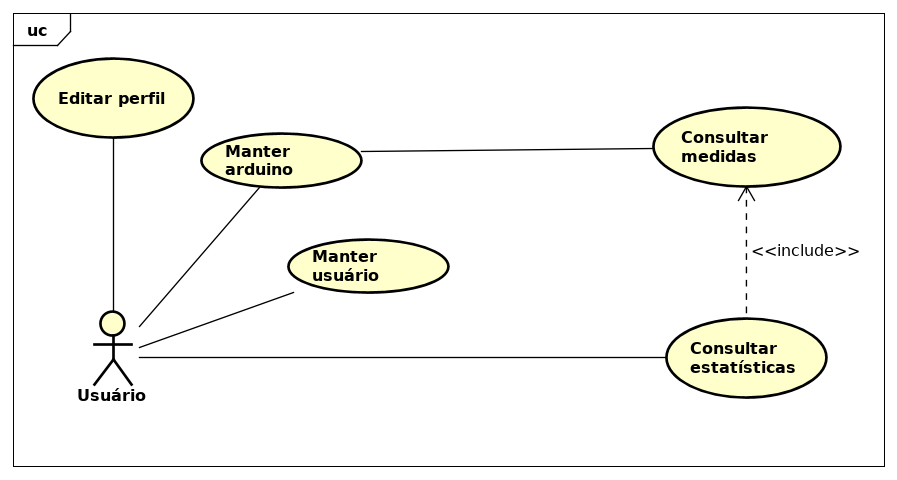
\includegraphics[scale=0.45]{diagrams/caso_de_uso.png}
    \hfill
\legend{Fonte: Produção do autor.}
\end{figure}

Através do diagrama do caso de uso contido na figura \ref{fig:figure_diagrama_caso_uso}, é possível identificar apenas um ator na aplicação, que é o usuário do sistema, interessado em visualizar informações geradas pela análise estatística dos dados capturados. O mesmo interage com a aplicação através da interface de usuário, realizando cadastros e consultas.

O requisito funcional \textbf{Consultar estatísticas} é o principal requisito do sistema, onde o usuário fará a filtragem dos dados, trazendo a ele as estatísticas geradas pela aplicação.
O usuário irá utilizar de campos de entrada de dados para escolher qual a estação meteorológica ele deseja visualizar, a data inicial para realizar as consultas, a data final e o intervalo de tempo para cálculo das médias.
Após a consulta das informações, o usuário irá obter como resultado as informações de mínimas e máximas das medidas e gráficos que o informam as médias para cada uma das propriedades meteorológicas.

O requisito funcional representado pelo caso de uso \textbf{Manter usuário}, descreve as ações do usuário acerca do cadastro de usuários no sistema.
Através desta funcionalidade, o usuário poderá, através da interface do usuário na web, utilizando tabelas, realizar o cadastro, consultas, atualização de informações e exclusão de usuários.
Durante a interação do usuário com a persistência de dados de usuários no sistema, caso erros ocorram, mensagens de erro auxiliares serão mostradas ao usuário, o auxiliando a encontrar qual o erro no processo realizado.

O requisito funcional \textbf{Manter arduino}, é muito similiar ao caso de uso anterior \textbf{Manter usuário}, e representa a persistência de informações acerca das estações meteorológicas no sistema, utilizando as quatro operações básicas de cadastro, consulta, atualização e exclusão de dados.

O requisito funcional de representado pelo caso de uso \textbf{Editar Perfil} representa a visualização e edição dos dados do usuário que está utilizando o sistema no momento, ele pode escolher editar suas informações, que exibe um formulário com os atuais dados preenchidos, onde o usuário pode realizar a alteração de suas informações.

\subsection{Detalhamento dos casos de uso}

Utilizando de tabelas, este capítulo descreve de forma detalhada cada um dos casos de uso, apresentado as descrições, os atores relacionados, as pré condições, exceções e fluxos alternativos, conforme pode ser visualizado nas tabelas de \ref{table:usecase_consultar_estatisticas} a \ref{table:usecase_edit_perfil}.

\begin{table}[H]
    \ABNTEXfontereduzida
    \caption{Consultar estatísticas}
    \label{table:usecase_consultar_estatisticas}
    \begin{tabularx}{\textwidth}{{l}|p{10.5cm}}

    \hline

    \multicolumn{2}{c}{\textbf{Realizar consultas com filtros}} \\

    \hline
    Descrição & Recebe do usuário os filtros para seleção das informações, então, realiza uma análise estatística dos dados requisitados e os exibe para o usuário utilizando listagens e gráficos. \\

    \hline

    Atores & Usuário \\

    \hline

    \multirow{3}{*}{Pré-condições} & Banco de dados em correto funcionamento \\
    & Filtros corretos passados pelo usuário \\
    & Listagem de estações meteorológicas retornando ao mínimo uma estação \\

    \hline

    \multirow{2}{*}{Exceções e fluxos alternativos} & Caso a seleção não retorne nenhuma informação ao usuário, uma mensagem de dados inexistentes é exibida \\
    & Em caso de perca de conexão com banco de dados, exibe uma mensagem de erro ao usuário \\
    & Caso não existam estações meteorológicas cadastradas, o filtro de seleção de estação meteorológica exibe um aviso ao usuário \\

    \hline

    \end{tabularx}
\end{table}

\begin{table}[H]
    \ABNTEXfontereduzida
    \caption{Especificações do caso de uso consultar medidas}
    \label{my-label}
    \begin{tabularx}{\textwidth}{{l}|p{10.5cm}}

    \hline

    \multicolumn{2}{c}{\textbf{Consultar medidas}} \\

    \hline
    Descrição & Consulta as medidas que estão persistidas no banco de dados para uma estação meteorológica, no software desenvolvido, atualmente este caso de uso é apenas acessado pela geração de estatísticas \\

    \hline

    \multirow{2}{*}{Pré-condições} & Credenciais de acesso ao banco de dados  \\
    & Banco de dados em correto funcionamento \\

    \hline

    \multirow{2}{*}{Exceções e fluxos alternativos} & Caso não existam medidas capturadas para a estação meteorológica, retorna uma lista vazia de dados \\

    \hline

    \end{tabularx}
\end{table}

\begin{table}[H]
    \ABNTEXfontereduzida
    \caption{Especificação do caso de uso manter usuários}
    \label{my-label}
    \begin{tabularx}{\textwidth}{{l}|p{10.5cm}}

    \hline

    \multicolumn{2}{c}{\textbf{Manter usuários}} \\

    \hline
    Descrição & Realiza uma listagem dos dados dos usuários atualmente registrados no sistema, fornecendo a possibilidade de cadastrar um novo usuário, atualizar os dados de um usuário ou excluir um usuário do sistema \\

    \hline

    \multirow{2}{*}{Pré-condições} & Credenciais de acesso ao banco de dados \\
    & Banco de dados em correto funcionamento \\

    \hline

    \multirow{2}{*}{Exceções e fluxos alternativos} & Caso não existam usuários cadastrados no sistema, exibe uma mensagem de aviso ao usuário \\
    & Para o cadastro ou atualização dos dados de um usuário, caso existam dados inválidos que foram dados como entrada, ao confirmar a operação, exibe uma mensagem de erro ao usuário \\

    \hline

    \end{tabularx}
\end{table}

\begin{table}[H]
    \ABNTEXfontereduzida
    \caption{Especificação do caso de uso manter estações meteorológicas}
    \label{my-label}
    \begin{tabularx}{\textwidth}{{l}|p{10.5cm}}

    \hline

    \multicolumn{2}{c}{\textbf{Manter estações meteorológicas}} \\

    \hline
    Descrição & Realiza uma listagem dos dados das estações meteorológicas atualmente registradas no sistema, fornecendo a possibilidade de cadastrar uma nova estação, atualizar os dados de uma estação ou excluir uma estação meteorológica do sistema \\

    \hline

    \multirow{2}{*}{Pré-condições} & Credenciais de acesso ao banco de dados  \\
    & Banco de dados em correto funcionamento \\

    \hline

    \multirow{2}{*}{Exceções e fluxos alternativos} & Caso não existam estações cadastradas no sistema, exibe uma mensagem de aviso ao usuário \\
    & Para o cadastro ou atualização dos dados de uma estação, caso existam dados inválidos que foram dados como entrada, ao confirmar a operação, exibe uma mensagem de erro ao usuário \\

    \hline

    \end{tabularx}
\end{table}

\begin{table}[H]
    \ABNTEXfontereduzida
    \caption{Especificação do caso de uso editar perfil}
    \label{table:usecase_edit_perfil}
    \begin{tabularx}{\textwidth}{{l}|p{10.5cm}}

    \hline

    \multicolumn{2}{c}{\textbf{Editar perfil}} \\

    \hline
    Descrição & Exibe os dados do usuário que está utilizando o sistema no momento, dando a possibilidade do usuário alterar os próprios dados \\

    \hline

    \multirow{2}{*}{Pré-condições} & Credenciais de acesso ao banco de dados  \\
    & Banco de dados em correto funcionamento \\

    \hline
    Exceções e fluxos alternativos & Caso na edição do perfil do usuário atual existam dados inválidos que foram dados como entrada, ao confirmar a operação, exibe uma mensagem de erro ao usuário \\

    \hline

    \end{tabularx}
\end{table}

\section{Requisitos não funcionais}

Os requisitos não funcionais, como seu próprio nome demonstra, não estão ligados diretamente ao que um software deve fazer, porém, tais requisitos são considerados tão importantes quanto os requisitos funcionais, pois podem comprometer a usabilidade e funcionalidades de um sistema \cite{engenharia_software_sommerville}.

Comumente, requisitos não funcionais estão ligados a questões de disponibilidade de software, tempo de resposta ao usuário e outras partes que se comunicam com o sistema e segurança.

Uma das formas de determinar a arquitetura do sistema seguindo os requisitos não funcionais é restringir a forma como as funcionalidades primárias do sistema trabalham, trabalhando no projeto e na implementação do software de forma restrita dentro destes padrões.

Nas seções subsequentes os tópicos de disponibilidade, tempo de resposta e segurança do sistema são melhor detalhados.

\subsection{Performance}

Para a boa usabilidade do usuário ao interagir com um sistema, um dos requisitos não funcionais mais importantes é o tempo de resposta de uma aplicação, pois, dependendo da lentidão com a qual as informações são disponibilizadas, um usuário pode ter problemas e, em muitos casos, não utilizar o sistema por conta do tempo de resposta.

Na era da informação, a informação é trabalhada de forma quase instantânea, portanto, tal requisito não pode ser deixado em segundo plano ao se trabalhar no projeto de um software.

No sistema desenvolvido, todo o desenvolvimento do sistema foi pensando de forma a fornecer ao usuário um baixo tempo de resposta através do uso de técnicas de desenvolvimento de software focadas em alta disponibilidade, desde a implementação da arquitetura do software e de como o banco de dados é utilizado, até a forma como os dados são carregados na interface do usuário. Para atingir tal objetivo, optou-se por disponibilizar ao usuário o mínimo de informações necessárias para a interação com o sistema.

Detalhes acerca da forma como o sistema é implementado para fornecer ao usuário a melhor experiência possível desde sua implementação em baixo nível são melhor descritos na seção sobre a arquitetura do software em \ref{sec:arquitetura_software}.

\subsection{Segurança}

Outro requisito muito importante para qualquer sistema é a segurança, tanto nas informações que ali estão contidas quanto no resultado final que é apresentado ao usuário, com a evolução da tecnologia, as pessoas passaram a estar muito mais próximas a sistemas de informação, colocando ali, informações sensíveis.

Neste projeto, para que se pudesse proporcionar ao usuário melhor segurança em seus dados e nas informações meteorológicas que são informadas, foram utilizadas técnicas de criptografia de informações, focando primariamente em informações que são sensíveis, e, para acesso ao sistema, técnicas de bloqueio de informações através de chaves foram utilizadas, melhores detalhes acerca de como tecnologias utilizadas funcionam são relatados na seção \ref{sec:arquitetura_software}, onde a arquitetura do software proposto é apresentada.

\section{Arquitetura macro}

A arquitura de um software segundo \citeauthoronline{engenharia_software_sommerville}, (\citeyear{engenharia_software_sommerville}):

\begin{citacao}
    É o elo crítico entre o projeto e a engenharia de requisitos, pois identifica os principais componentes estruturais de um sistema e os relacionamentos entre eles. O resultado do processo de projeto de arquitetura é um modelo de arquitetura que descreve como o sistema está organizado em um conjunto de componentes de comunicação. (p.104).
\end{citacao}

Procurando descrever os casos de uso do sistema, optou-se por utilizar uma descrição da arquitetura macro do software através de figuras, descrevendo o todo do sistema através de simples componentes, pode-se conferir a arquitetura através da figura \ref{fig:figure_arq_macro}

\begin{center}
\begin{figure}[H]
    \centering
    \caption{Representação da arquitetura} \label{fig:figure_arq_macro}
    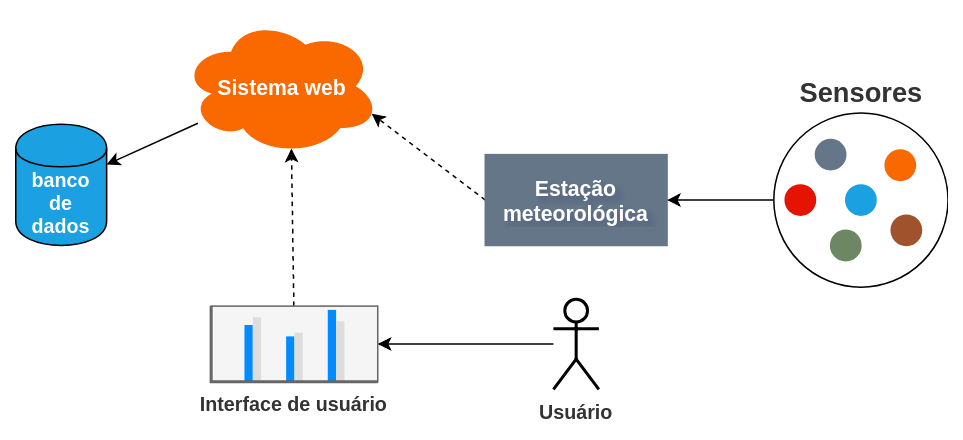
\includegraphics[scale=0.43]{diagrams/arq_macro.png}
    \hfill
\legend{Fonte: Produção do autor.}
\end{figure}
\end{center}

Através do desenho da arquitetura do software pode-se identificar as relações entre os diversos componentes do sistema, porém, de uma forma a qual a qual as partes interessadas no projeto ainda podem interagir e entender o que está sendo proposto.

No diagrama, pode-se identificar os sensores conectados diretamente com a estação meteorológica (traço preenchido), enviando as informações capturadas para a estação meteorológica através de conexão web (traço pontilhado), que, após receber as informações as envia para o sistema Web, que as persiste em banco de dados.

O usuário, interage com o sistema diretamente através da interface que disponibiliza gráficos para que o acompanhamento possa ser realizando, consultando as informações através de conexão web com o sistema.

Dessa forma, pode-se descrever a arquitetura do projeto, visando, atingir o objetivo definido através da engenharia de requisitos com um projeto agora melhor detalhado, tanto para as partes interessadas, quanto para a equipe de software, nas seções seguintes, é descrita de forma técnicas os componentes do sistema, através de diagramas UML.

\chapter{Diagramas do sistema}

Foram utilizados para a descrição dos componentes da aplicação os diagramas UML, os diagramas de classe, de sequência e de estado descrevem o software nos capítulos seguintes.

\section{Diagrama de classes}

"Os diagramas de classe são usados no desenvolvimento de um modelo de sistema orientado a objetos para mostrar as classes de um sistema e as associações entre essas classes. Em poucas palavras, uma classe de objeto pode ser pensada como uma definição geral de um tipo de objeto do sistema." \cite{engenharia_software_sommerville}.

O sistema desenvolvido implementa o paradigma de programação funcional de forma pouco restrita, portanto, alguns conceitos de programação orientada a objetos foram descartados. Porém, o diagrama de classes também pode representar as características das entidades do sistema.

\begin{center}
\begin{figure}[H]
    \centering
    \caption{Diagrama de classes \label{fig:figure_diagrama_classe}}
    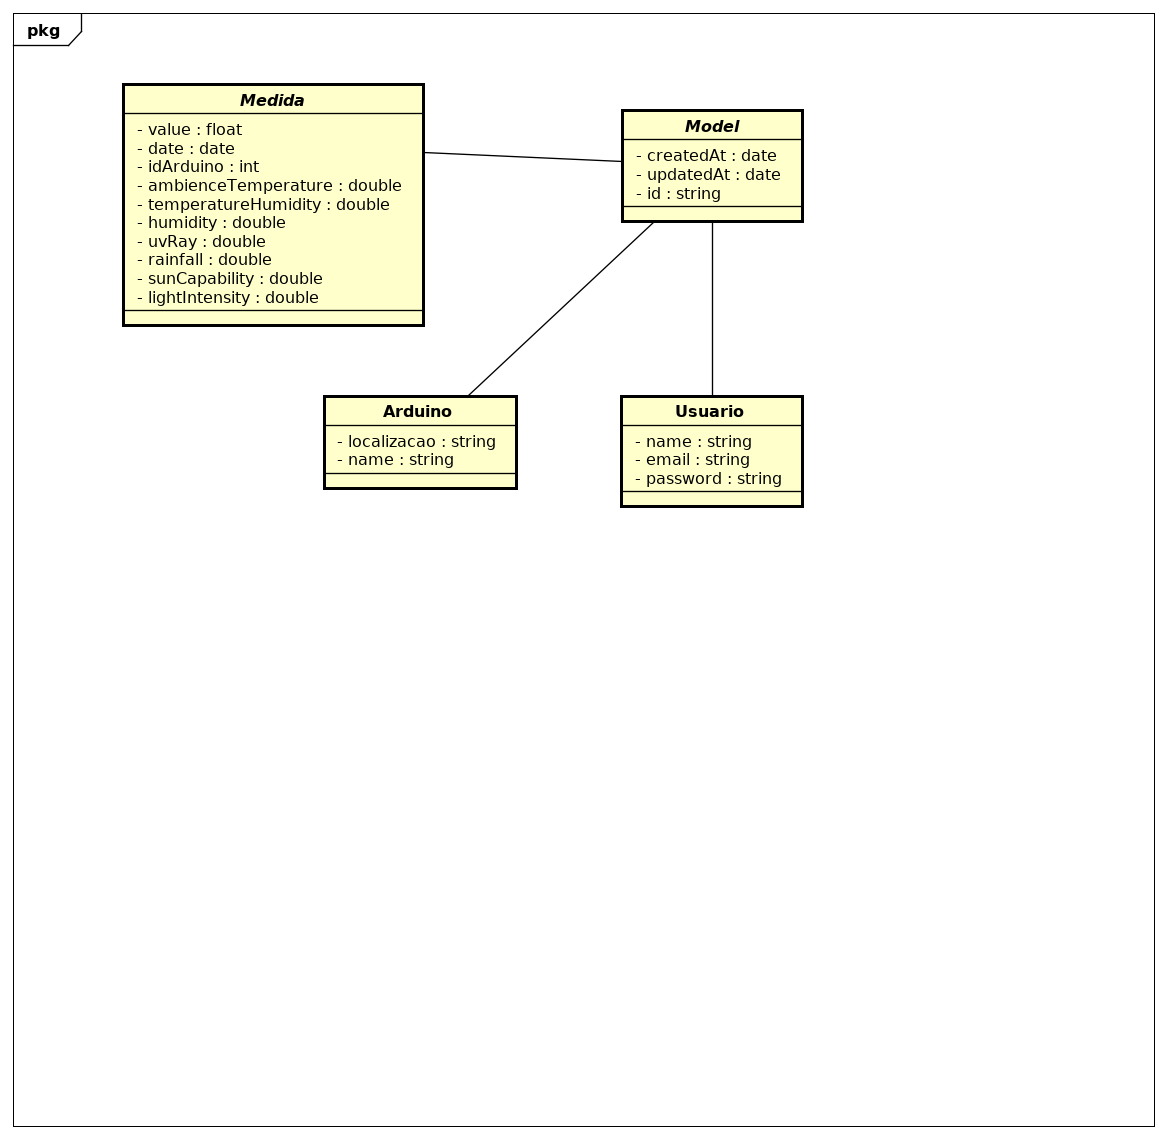
\includegraphics[scale=0.5]{diagrams/classe.png}
    \hfill
\legend{Fonte: Produção do autor.}
\end{figure}
\end{center}

Como se pode verificar no diagrama descrito na figura \ref{fig:figure_diagrama_classe} as entidades do sistema consistem na medida, que é a informação que foi capturada pela estação meteorológica, que pertence a uma estação, a entidade de estação meteorológica, que possui nenhuma a muitas medidas capturadas, e a entidade de usuário, que representa um usuário cadastrado no sistema.

As propriedades de cada entidade são especificadas nas figuras \ref{fig:spec_model_base} a \ref{fig:spec_model_user}, descartando seus comportamentos, pois, as mesmas são manipuladas através das camadas, que são descritas nas seções que descrevem o comportamento do sistema, através de diagramas de sequência e estado, nas respectivas seções \ref{sec:diagrama_sequencia} e \ref{sec:diagrama_estado}.

\begin{center}
\centering
\begin{table}[H]
    \ABNTEXfontereduzida
    \caption{Especificação da Model base \label{fig:spec_model_base}}
    \begin{tabularx}{\textwidth}{{l}|p{13.4cm}}

    \hline

    \multicolumn{2}{c}{\textbf{Model}} \\

    \hline
    Descrição & É a model base da aplicação, que advem do framework utilizado pra mapeamento dos objetos para o banco de dados \\

    \hline

    \multicolumn{2}{c}{Propriedades} \\

    \hline
    id & Identifica de forma única um objeto no banco de dados \\

    \hline
    createdAt & Data em que o objeto foi armazenado \\

    \hline
    updatedAt & Data em que alguma das propriedades do objeto foi alterada pela última vez \\

    \hline

    \end{tabularx}
\end{table}
\end{center}

\begin{center}
    \centering
    \begin{table}[H]
        \ABNTEXfontereduzida
        \caption{Especificação da Medida}
        \label{my-label}
        \begin{tabularx}{\textwidth}{{l}|p{11.66cm}}
    
        \hline
    
        \multicolumn{2}{c}{\textbf{Medida}} \\
    
        \hline
        Descrição & Representada a medida que foi capturada pela estação meteorológica \\
    
        \hline
    
        \multicolumn{2}{c}{Propriedades} \\
    
        \hline
        idArduino & Identificação do arduino que realizou a captura \\
    
        \hline
        ambienceTemperatura & O valor que foi capturado pelo sensor de temperatura ambiente \\
    
        \hline
        temperatureHumidity & Valor da temperatura capturada pelo sensor agregado de temperatura e umidade \\

        \hline
        humidity & Valor da umidade capturada pelo sensor agregado de temperatura e umidade \\

        \hline
        uvRay & Nível de radiação uv que foi medida \\
        
        \hline
        rainfall & Porcentagem de chuva capturada \\

        \hline
        sunCapability & Capacidade solar que foi medida \\

        \hline
        lightIntensity & Nível da intensidade de luz capturada \\
    
        \hline
    
        \end{tabularx}
    \end{table}
\end{center}

\begin{center}
    \centering
    \begin{table}[H]
        \ABNTEXfontereduzida
        \caption{Especificação da Estação Meteorológica}
        \label{my-label}
        \begin{tabularx}{\textwidth}{{l}|p{13.6cm}}
    
        \hline
    
        \multicolumn{2}{c}{\textbf{Estação meteorológica}} \\
    
        \hline
        Descrição & Representa uma estação meteorológica cadastrada no sistema \\
    
        \hline
    
        \multicolumn{2}{c}{Propriedades} \\
    
        \hline
        location & Descrição de onde a estação meteorológica está posicionada \\

        \hline
        name & Nome de identificação da estação meteorológica \\
    
        \hline
    
        \end{tabularx}
    \end{table}
\end{center}

\begin{center}
    \centering
    \begin{table}[H]
        \ABNTEXfontereduzida
        \caption{Especificação do Usuário \label{fig:spec_model_user}}
        \begin{tabularx}{\textwidth}{{l}|p{13.60cm}}
    
        \hline
    
        \multicolumn{2}{c}{\textbf{Usuário}} \\
    
        \hline
        Descrição & Representa um usuário cadastrado no sistema \\
    
        \hline
    
        \multicolumn{2}{c}{Propriedades} \\
    
        \hline
        name & Nome de identificação do usuário \\

        \hline
        email & E-mail que identifica o usuário e é utilizado para login no sistema \\

        \hline
        password & Senha do usuário ao acessar o sistema, a informação é criptografada \\
    
        \hline
    
        \end{tabularx}
    \end{table}
\end{center}

\section{Diagrama de sequência}
\label{sec:diagrama_sequencia}

"Os diagramas de sequência em UML são usados, principalmente, para modelar as interações entre os atores e
os objetos em um sistema e as interações entre os próprios objetos. A UML tem uma sintaxe rica para diagramas
de sequência, que permite a modelagem de vários tipos de interação." \cite{engenharia_software_sommerville}.

Nesta seção, é apresentado o diagrama de sequência que representa o armazenamento de uma medida capturada por uma estação meteorológica, apresentando desde a saída dos dados, até a sua persistência em banco.

Para melhor aproveitamento da estação meteorológica e para que não haja necessidade de espera de uma resposta do software, utilizou-se da programação assíncrona para responder com sucesso a estação, os dados são enviados, e uma resposta de sucesso é emitido a estação, porém, os dados são processados em seguida, deixando livre a fila de envio na estação.

\begin{figure}[H]
    \centering
    \caption{Diagrama de sequência \label{fig:figure_diagrama_sequencia}}
    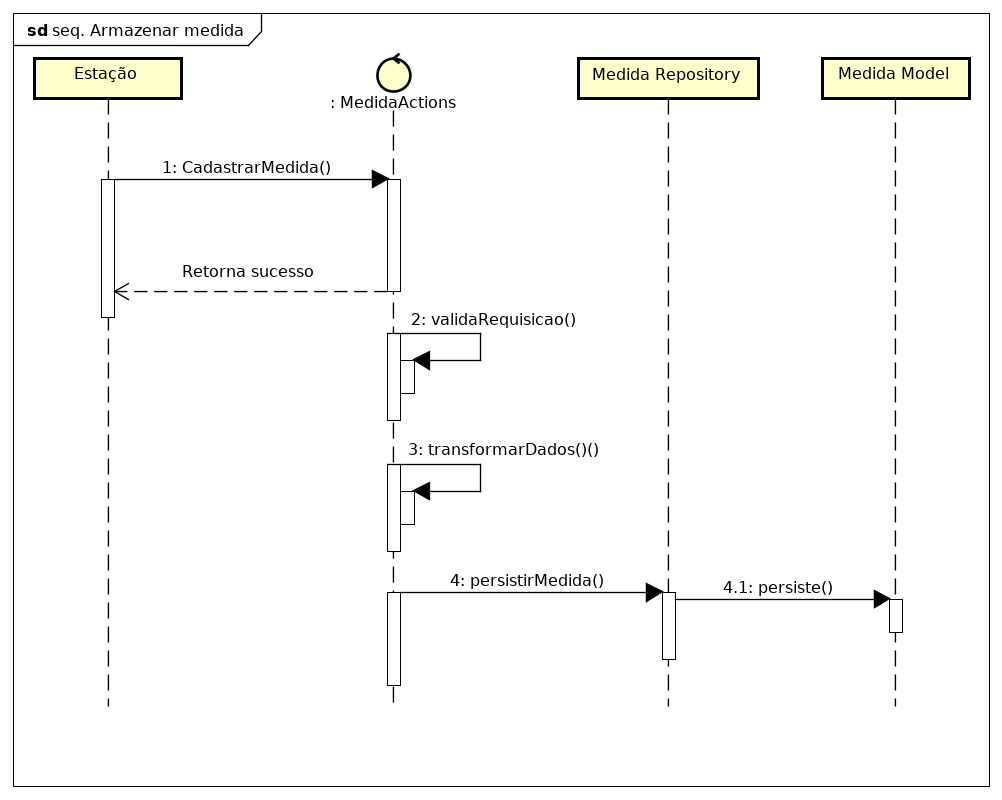
\includegraphics[scale=0.40]{diagrams/sequencia.png}
    \hfill
\legend{Fonte: Produção do autor.}
\end{figure}

Como descrito no diagrama de sequência representado na figura \ref{fig:figure_diagrama_sequencia} a aplicação é composta por 3 principais camadas, seguindo um modelo que são descritas nos capítulos seguintes.

\subsection{Controlador}

Na camada de controle, após ser recebida uma mensagem da estação meteorológica, a mesma retorna sucesso para a estação, porém sem a confirmação das informações, que são logo em seguida, validadas, e então são tratadas utilizando as regras descridas na seção \ref{sec:tratamento_dados}.

\subsection{Repositório}

A camada de repositório trabalha como uma intermediaria entre o controlador da aplicação onde a validação dos dados é feita e a camada de persistência da aplicação, ela trabalha verificando se os dados persistidos estão corretos e fornece um local comum para consulta e armazenamento das informações.

\subsection{Modelo}

A camada de modelos, é composta pelas entidades do sistema, é a única camada da aplicação que possui acesso direto ao banco de dados, e é gerenciada através da ferramenta de comunicação com o banco de dados, abstraindo assim, o acesso ao baixo nível da persistência do software.

\section{Diagrama de estado}
\label{sec:diagrama_estado}

"O diagrama de máquina de estados demonstra o comportamento de um elemento por meio de um conjunto finito de transições de estado, ou seja, uma máquina de estados." \cite{uml_pratica}.

O diagrama de estado abaixo compreende a consulta de estatísticas na aplicação, demonstrando, o estado de uma requisição no sistema até sua resposta ao usuário.

\begin{center}
\begin{figure}[H]
    \centering
    \caption{Diagrama de estado \label{fig:figure_diagrama_estado}}
    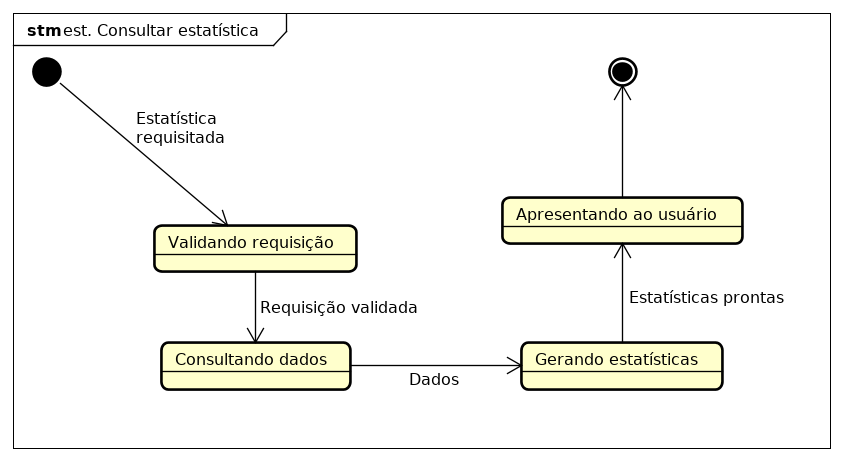
\includegraphics[scale=0.50]{diagrams/estado.png}
    \hfill
\legend{Fonte: Produção do autor.}
\end{figure}
\end{center}

Na figura 5 pode-se identificar os estados como sendo a estatística requisitada ao sistema, a requisição sendo identificada como válido, então, os dados são encontrados no sistema e as estatísticas são apresentadas ao usuário.

No estado identificado como \textbf{Validando requisição}, a mesma é validada, identificando se o usuário realmente possui acesso ao sistema e se os filtros que foram aplicados são também válidos, após os dados são consultados e passados para a geração de estatísticas, nos estados \textbf{Consultando dados} e \textbf{Gerando estatísticas}, respectivamente, por fim, no estado identificado como \textbf{Apresentando ao usuário} os gráficos são renderizados na tela, e o ciclo de vida da requisição termina.

\chapter{Arquitetura das estações meteorológicas}

Para a construção da arquitetura da estação meteorológica, foi utilizado como central o microcontrolador arduino, diversos sensores para captura das informações e a placa WiFi NodeMCU para conexão a internet e gerenciamento das requisições com o servidor.

\section{Arduino}
\label{sec:arduino}

Como definido em seu site oficinal: "O Arduino é uma plataforma eletrônica de código aberto baseada em hardware e software de fácil utilização. É destinado a qualquer pessoa que construa projeto interativos." \cite{arduino_about}.

Ele fornece um controlador eletrônico único baseado no microprocessador ATmega328, desenvolvido em c++, componentes eletrônicos oficinais para a construção de aplicações interativas e uma IDE (Ambiente de desenvolvimento integrado) para a construção de sistemas.

Para a construção da estação meteorológica descrita, foi utilizado arduino UNO, em sua versão contendo 6 portas analógicas, 6 portas digitais uma cpu com velocidade de 16 MHz e 32 KB de armazenamento interno.

Foram utilizados diversos sensores conectados as portas seriais do arduino para coleta de dados, após coletados os dados, o arduino monta a requisição que o servidor espera em formato JSON, é um formato de dados similar ao XML, porém, utiliza a sintaxe de objetos do javascript, para a construção do JSON não foi utilizada nenhuma biblioteca, por conta da quantidade de memória limitada do arduino.

Na figura \ref{fig:arduino_diagram}, pode-se conferir o diagrama da estação meteorológica, demonstrando de forma resumida a ligação entre os sensores, o arduino e o nodeMCU.

\begin{figure}[H]
    \centering
    \caption{Esboço da estação meteorológica \label{fig:arduino_diagram}}
    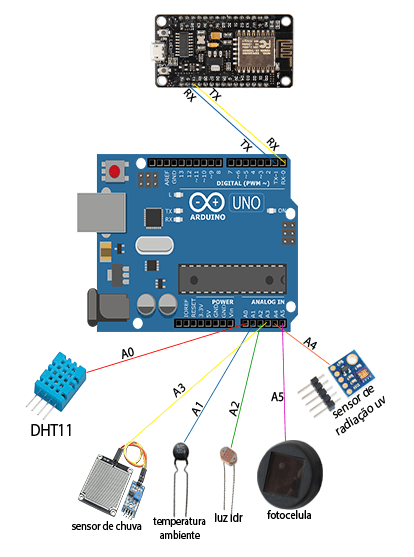
\includegraphics[scale=0.8]{diagrams/arduino.png}
    \hfill
\legend{Fonte: Produção do autor.}
\end{figure}

Na figura \ref{fig:arduino_prototipo} pode-se visualizar o protótipo construído.

\begin{figure}[H]
    \centering
    \caption{Protótipo da estação meteorológica \label{fig:arduino_prototipo}}
    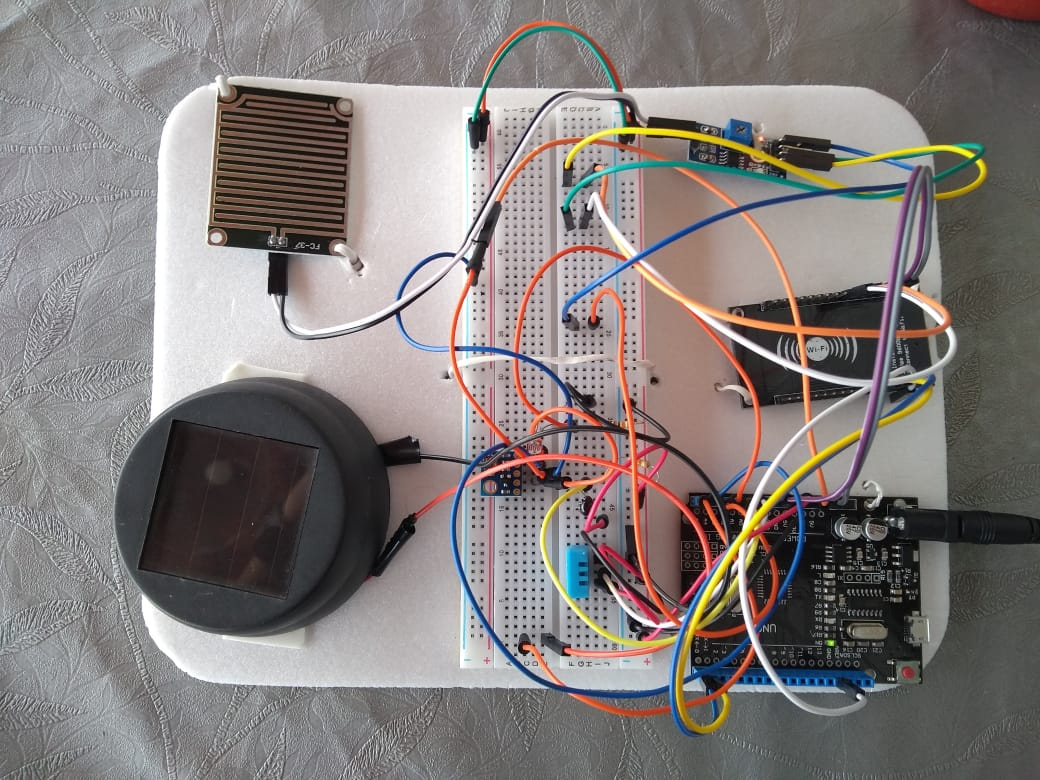
\includegraphics[scale=0.4]{arduino_prototipo.jpeg}
    \hfill
\legend{Fonte: Produção do autor.}
\end{figure}

\section{Sensores}
\label{sec:sensores}

Para a captura das informações foram utilizados os sensores de temperatura, umidade do ar com temperatura em relação a umidade, sensor de chuva digital/analógico, sensor de intensidade luminosa, radiação UV e capacidade solar.

Os sensores utilizados se conectam com o arduino através de suas portas seriais, emitindo as informações nas portas seriais para que o arduino possa as capturar.

Os sensores utilizados são melhor descritos nas tabelas de descrição \ref{table:dht11} a \ref{table:sensor_uv}.

\begin{center}
    \centering
    \begin{table}[H]
        \ABNTEXfontereduzida
        \caption{Especificação do sensor de umidade e temperatura em relação a umidade \label{table:dht11}}
        \begin{tabularx}{\textwidth}{{l}|p{13.1cm}}
    
        \hline
    
        \multicolumn{2}{c}{\textbf{Sensor de umidade e temperatura relativa DHT11}} \\
    
        \hline
        Descrição & Capturam os valores de umidade e temperatura em relação a umidade \\
    
        \hline
    
        Conexão & Se conecta com o arduino através da porta análogica 0 (A0) \\

        \hline

        \multicolumn{2}{c}{Identificação dos valores} \\
    
        \hline
        Umidade & É representada por porcentagem (0 a 100\%) \\

        \hline
        Temperatura & Capta a temperatura atual em $^\circ$C \\
    
        \hline
    
        \end{tabularx}
    \end{table}
\end{center}

\begin{center}
    \centering
    \begin{table}[H]
        \ABNTEXfontereduzida
        \caption{Especificações do sensor de temperatura ambiente}
        \label{my-label}
        \begin{tabularx}{\textwidth}{{l}|p{13.1cm}}
    
        \hline
    
        \multicolumn{2}{c}{\textbf{Sensor de temperatura ambiente Thermistor}} \\
    
        \hline
        Descrição & Captura o valor da temperatura ambiente \\
    
        \hline
    
        Conexão & Se conecta com o arduino através da porta analógica 1 (A1) \\

        \hline

        \multicolumn{2}{c}{Identificação dos valores} \\

        \hline
        Temperatura & Capta a temperatura ambiente atual em $^\circ$C \\
    
        \hline
    
        \end{tabularx}
    \end{table}
\end{center}

\begin{center}
    \centering
    \begin{table}[H]
        \ABNTEXfontereduzida
        \caption{Especificações do sensor de luminosidade LDR}
        \label{my-label}
        \begin{tabularx}{\textwidth}{{l}|p{13.4cm}}
    
        \hline
    
        \multicolumn{2}{c}{\textbf{Sensor de luminosidade LDR}} \\
    
        \hline
        Descrição & Captura o valor da intensidade luminosa \\
    
        \hline
    
        Conexão & Se conecta com o arduino através da porta analógica 2 (A2) \\

        \hline

        \multicolumn{2}{c}{Identificação dos valores} \\

        \hline
        < 100 & Claridade Intensa \\
        
        \hline
        100 - 300 & Claridade alta \\
        
        \hline
        300 – 500 & Claridade acima da média \\
        
        \hline
        500 – 700 & Claro \\
        
        \hline
        700 - 850 & Pouca Claridade \\
        
        \hline
        850 - 1000 & Muito Pouca Claridade \\
        
        \hline
        > 1000 & Escuro \\
    
        \hline
    
        \end{tabularx}
    \end{table}
\end{center}

\begin{center}
    \centering
    \begin{table}[H]
        \ABNTEXfontereduzida
        \caption{Especificações do sensor de nível de chuva}
        \label{my-label}
        \begin{tabular*}{\textwidth}{{l}|p{13.5cm}}
    
        \hline
    
        \multicolumn{2}{c}{\textbf{Sensor de chuva}} \\
    
        \hline
        Descrição & Captura através do sensor digital se está chovendo (1) ou não (0) e através do sensor análogico de 0 a 4.5 \\
    
        \hline
    
        Conexão & Se conecta com o arduino através da porta analógica 3 (A3) \\

        \hline

        \multicolumn{2}{c}{Identificação dos valores} \\

        \hline
        < 2.00      & Sem Chuva \\

        \hline
        2.00 – 3.00 & Nuvens Esparsas \\

        \hline
        3.00 – 3.99 & Nublado \\

        \hline
        4.00 – 4.50 & Chuva \\

        \hline
        > 4.50      & Chuva Intensa \\
    
        \hline
    
        \end{tabular*}
    \end{table}
\end{center}

\begin{center}
    \centering
    \begin{table}[H]
        \ABNTEXfontereduzida
        \caption{Especificações do sensor de capacidade solar}
        \label{my-label}
        \begin{tabularx}{\textwidth}{{l}|p{13.5cm}}
    
        \hline
    
        \multicolumn{2}{c}{\textbf{Sensor de capacidade solar}} \\
    
        \hline
        Descrição & Captura a capacidade solar utilizando fotocélula \\
    
        \hline
    
        Conexão & Se conecta com o arduino através da porta analógica 5 (A5) \\

        \hline

        \multicolumn{2}{c}{Identificação dos valores} \\

        \hline
        < 1,00      & Fraca \\

        \hline
        1,00 – 1,49 & Média \\

        \hline
        1,50 – 1,99 & Boa \\

        \hline
        >= 2,00     & Ótima \\
    
        \hline
    
        \end{tabularx}
    \end{table}
\end{center}

\begin{center}
    \centering
    \begin{table}[H]
        \ABNTEXfontereduzida
        \caption{Especificações do sensor de radiação uv \label{table:sensor_uv}}
        \begin{tabularx}{\textwidth}{p{5cm}|c|c|c|c|c|c}
    
        \hline
    
        \multicolumn{7}{c}{\textbf{Sensor de radiação uv}} \\

        \hline
        \multicolumn{1}{c}{Descrição} & \multicolumn{6}{c}{Captura índice uv de forma analógica (0 - 240)}  \\
    
        \hline
        \multicolumn{1}{c}{Conexão} & \multicolumn{6}{c}{Se conecta com o arduino através da porta analógica 4 (A4)} \\

        \hline

        \multicolumn{7}{c}{Identificação dos valores} \\

        \hline
        \centering{Índice UV} & 0 & 1 & 2 & 3 & 4 & 5 \\

        \hline
        \centering{Voltagem (mV)} & <50 & 227 & 318 & 408 & 503  & 606 \\

        \hline
        \centering{Valor analógico} & <10 & 46 & 65 & 83 & 103 & 124 \\

        \hline
        \centering{Índice UV} & 6   & 7   & 8   & 9   & 10   & 11+  \\

        \hline
        \centering{Voltagem (mV)} & 696 & 795 & 881 & 976 & 1079 & 1170 \\

        \hline
        \centering{Valor analógico} & 142 & 162 & 180 & 200 & 221 & 240 \\
    
        \hline
    
        \end{tabularx}
    \end{table}
\end{center}

Alguns dados foram tratados antes de serem armazenados em banco de dados, detalhes acerca da transformação de dados que foi aplicada são melhor abordados na seção \ref{sec:tratamento_dados}.

\section{NodeMCU}
\label{sec:nodemcu}

Para a conexão e envio dos dados para o servidor, foi utilizada a placa wifi NodeMCU ESP8266, conectada nas portas TX e RX.

A placa NodeMCU fornece possibilidade de conexão com rede wifi e roteamento wifi e pode ser programada em linguagem LUA ou utilizando a IDE do Arduino.

No projeto, o arduino se conecta com o NodeMCU através das portas TX e RX, onde o NodeMCU espera que os dados que foram capturados pelo Arduino são escritos em sua porta serial, então, os dados são enviados através de requisição HTTP para o servidor.

As configurações da placa NodeMCU são definidas no começo de seu arquivo de código fonte (linhas 3 - 12).

\chapter{Arquitetura do software}
\label{sec:arquitetura_software}

Segundo \citeauthoronline{clean_architecture}, um dos maiores pensadores sobre o assunto da qualidade de software na modernidade, em seu livro Clean Architecture (Arquitetura limpa): "O software foi inventado para ser soft”. Pretendia ser uma maneira de alterar facilmente o comportamento das máquinas. Se quiséssemos que o comportamento das máquinas fosse difícil de mudar, teríamos chamado de hardware". \cite{clean_architecture}.

A arquitetura de software desenvolvida utiliza da separação dos componentes de software em pacotes que são exportados e podem ser utilizados em qualquer parte da aplicação, separando as responsabilidades do sistema, utilizando também os benefícios de técnicas do paradigma de programação funcional, foi possível isolar os pontos de efeitos colaterais da aplicação, deixando os comportamentos da aplicação, mais previsíveis.

Para a construção, foi utilizado clássico modelo de cliente servidor, onde a aplicação do lado cliente tem a responsabilidade de renderizar o que o cliente vê (front end) e a aplicação no lado servidor tem a responsabilidade de aplicar regras de negócio, realizar armazenamento e análise dos dados solicitados (back end), no sistema construído, o lado cliente e o lado servidor se comunicam através de protocolo HTTP, utilizando o conceito restful no lado servidor que é descrito na seção \ref{sec:servidor} e o lado cliente utiliza a tecnologia SPA (Single Page Application), que é detalhada na seção \ref{sec:cliente}

\section{Servidor}
\label{sec:servidor}

O lado do servidor foi construído utilizando NodeJS, um runtime para Javascript no lado servidor, foi disponibilizada para a aplicação uma API (Application Programming Interface) via HTTP para a comunicação tanto da interface do usuário quanto para o arduino, utilizando os métodos RESTful.
Uma RESTful API é uma interface de acesso a aplicação aplicação que utiliza requisições http para a criação, atualização, consulta e exclusão de dados \cite{restful_api}. No sistema desenvolvido, foi utilizado o formato de dados JSON.

A documentação da api pode ser conferida na seção \ref{sec:doc_api}.

\subsection{Banco de dados}

O banco de dados utilizado foi o MongoDB, um banco de dados não relacional, o desenho do banco de dados é controlado pela aplicação, que define quis campos devem ser indexados e como os dados devem se "relacionar", cada informação capturada fica armazenada dentro de uma coleção, utilizando o formato JSON.

A escolha de um banco de dados não relacional, foi motivada pela facilidade ao se trabalhar com esquemas maleaveis, podendo ter suas informações mutadas, deixando a cargo da aplicação a tomada de decisão.

O banco MongoDB foi escolhido pela sua facilidade ao trabalhar com escrita de dados concorrente, pois, as informações são, em primeiro instante processadas e armazenadas em cache, e já são retornadas para a aplicação, somente após, o MongoDB se encarrega de realizar a inserção dos dados em disco.

Com todas as vantagens do banco de dados, a aplicação tira vantagem, se beneficiando no que toca performance, disponibilidade e mutabilidade das informações.

\subsection{Tratamento dos dados meteorológicos}
\label{sec:tratamento_dados}

Os dados que foram capturados pelas estações, tiveram seus valores mantidos, com exceção dos valores de intensidade de luz e quantidade de chuva, o valor de intensidade de luz precisou ser invertido para melhor visualização das informações.

Para a medição de intensidade de luz considerando $x$ como o valor que foi capturado, com sua máxima identificada como $1024$, a equação $1024 - x$ é aplicada, invertendo o valor, caso o resultado seja negativo, o valor $0$ é considerado em seu lugar, para a quantidade de chuva, a mesma regra foi aplicada, porém, o valor também foi convertido para \%, então a fórmula para obtenção do valor que será armazenado para quantidade de chuva será $((1024-x)/1024)100$, novamente, dado resultado negativo, será considerada a porcentagem $0$.

\subsection{Análise dos dados}

São retornados ao usuário os dados de médias, mínimas e máximas, por serem os valores mais significantes para o acompanhamento meteorológico na situação identificada.
Para obtenção das médias dos valores, foi aplicada a função de agregação do MongoDB, reunindo as informações por intervalo de tempo e aplicando a função de média sobre o resultado.

\subsection{Documentação da API}
\label{sec:doc_api}

Na tabela \ref{table:table_api_routes} são detalhadas as rotas da api, documentando os métodos que foram utilizados, os endereços de cada uma das rotas e sua descrição.

\begin{table}[H]
    \centering
    \caption{Descrição das rotas da API}
    \label{table:table_api_routes}
    \begin{tabularx}{\textwidth}{l|l|l}
    \hline
    \textbf{Método}  & \textbf{Rota}        & \textbf{Descrição}                           \\ \hline
    GET              & /arduino             & Lista os arduinos                            \\ \hline
    GET              & /arduino/:id         & Retorna os dados de um arduino               \\ \hline
    POST             & /arduino             & Cadastra um novo arduino                     \\ \hline
    POST, PATCH, PUT & /arduino/:id         & Atualiza os dados de um arduino              \\ \hline
    DELETE           & /arduino/:id         & Deleta um arduino e suas medidas capturadas  \\ \hline
    GET              & /user                & Lista os usuários                            \\ \hline
    GET              & /user/:id            & Retorna os dados de um usuário               \\ \hline
    POST             & /user                & Cadastra um novo usuário                     \\ \hline
    POST, PATCH, PUT & /user/:id            & Atualiza os dados de um usuário              \\ \hline
    DELETE           & /user/:id            & Deleta um usuário                            \\ \hline
    POST             & /user/login          & Recebe as credenciais e retorna o token      \\ \hline
    POST             & /measure             & Cadastra uma medida capturada                \\ \hline
    GET              & /statistic/:id       & Retorna as estatísticas de dados do arduino  \\ \hline
    \end{tabularx}
\end{table}

Nas tabelas \ref{table:get_arduino} a \ref{table:get_statistic}, se pode conferir o detalhamento de cada uma das rotas da API, para todos os casos, os dados que forem retornados da API, são encapsulados na variável data dentro do corpo de resposta da requisição HTTP, no caso de listagem de dados, a variável data é um vetor que armazena as entidades listadas e no retorno de uma única entidade, a variável data é um objeto contendo os dados que foram retornados.

Juntamente com os dados, o campo success é retornado, quando verdadeiro, a requisição foi processada com sucesso, caso contrário, a requisição foi processada sem sucesso. Para todos os retornos, considere também os campos adicionais informados na tabela \ref{table:campos_adicionais}.

\begin{table}[H]
    \centering
    \caption{Especificações das rotas de listagem e retorno de arduino \label{table:get_arduino}}
    \begin{tabular}{c|c|c}
    \hline
    \multicolumn{3}{c}{\textbf{GET /arduino e GET /arduino/:id}} \\ \hline
    \multicolumn{3}{c}{Saída}                                                          \\ \hline
    \textbf{Propriedade}         & \textbf{Tipo}         & \textbf{Descrição}            \\  \hline
    name                         & String                & Nome da estação               \\  \hline
    location                     & String                & Localização da estação \\

    \hline
    \end{tabular}
\end{table}

\begin{table}[H]
    \centering
    \caption{Descrição dos campos adicionais \label{table:campos_adicionais}}
    \begin{tabular}{c|c|c}
    \hline
    \multicolumn{3}{c}{\textbf{Campos adicionais}} \\ \hline
    \textbf{Propriedade}         & \textbf{Tipo}         & \textbf{Descrição}            \\  \hline
    \_id                         & String                & Identificador da entidade no banco de dados      \\  \hline
    createdAt                    & String                & Data de inserção do registro no banco de dados         \\ \hline
    updatedAt                    & String                & Data da última atualização em dados do registro         \\ \hline
    \end{tabular}
\end{table}

\begin{table}[H]
    \centering
    \caption{Especificações das rotas de atualização e cadastro de arduino}
    \begin{tabular}{c|c|c}
    \hline
    \multicolumn{3}{c}{\textbf{POST /arduino e POST /arduino/:id}} \\ \hline
    \multicolumn{3}{c}{Entrada}                                                        \\ \hline
    \textbf{Propriedade}         & \textbf{Tipo}         & \textbf{Descrição}            \\  \hline
    name                         & String                & Nome da estação               \\  \hline
    location                     & String                & Localização da estação \\

    \hline

    \multicolumn{3}{c}{Saída}                                                        \\ \hline
    \textbf{Propriedade}         & \textbf{Tipo}         & \textbf{Descrição}            \\  \hline
    name                         & String                & Nome da estação               \\  \hline
    location                     & String                & Localização da estação \\

    \hline
    \end{tabular}
\end{table}

\begin{table}[H]
    \centering
    \caption{Especificações da rota exclusão de arduino}
    \begin{tabular}{c|c|c}
    \hline
    \multicolumn{3}{c}{\textbf{DELETE /arduino/:id}} \\ \hline
    \multicolumn{3}{c}{Saída}                                                          \\ \hline
    \textbf{Propriedade}         & \textbf{Tipo}         & \textbf{Descrição}            \\  \hline
    name                         & String                & Nome da estação               \\  \hline
    location                     & String                & Localização da estação \\

    \hline
    \end{tabular}
\end{table}

\begin{table}[H]
    \centering
    \caption{Especificações das rotas de listagem e retorno de usuário}
    \begin{tabular}{c|c|c}
    \hline
    \multicolumn{3}{c}{\textbf{GET /user e GET /user/:id}} \\ \hline
    \multicolumn{3}{c}{Saída}                                                          \\ \hline
    \textbf{Propriedade}         & \textbf{Tipo}         & \textbf{Descrição}            \\  \hline
    name                         & String                & Nome do usuário               \\  \hline
    email                        & String                & E-mail do usuário \\
    \hline
    password                     & String                & Senha criptografada do usuário \\
    \hline
    \end{tabular}
\end{table}

\begin{table}[H]
    \centering
    \caption{Especificações das rotas de atualização e cadastro de usuário}
    \begin{tabular}{c|c|c}
    \hline
    \multicolumn{3}{c}{\textbf{POST /user e POST /user/:id}} \\ \hline
    \multicolumn{3}{c}{Entrada}                                                        \\ \hline
    \textbf{Propriedade}         & \textbf{Tipo}         & \textbf{Descrição}            \\  \hline
    name                         & String                & Nome do usuário               \\  \hline
    email                        & String                & E-mail do usuário \\
    \hline
    password                     & String                & Senha do usuário \\

    \hline

    \multicolumn{3}{c}{Saída}                                                        \\ \hline
    \textbf{Propriedade}         & \textbf{Tipo}         & \textbf{Descrição}            \\  \hline
    name                         & String                & Nome do usuário               \\  \hline
    email                        & String                & E-mail do usuário \\
    \hline
    password                     & String                & Senha criptografada do usuário \\

    \hline
    \end{tabular}
\end{table}

\begin{table}[H]
    \centering
    \caption{Especificações da rota de login de usuário}
    \begin{tabular}{c|c|c}
    \hline
    \multicolumn{3}{c}{\textbf{POST /user/login}} \\ \hline
    \multicolumn{3}{c}{Entrada}                                                        \\ \hline
    \textbf{Propriedade}         & \textbf{Tipo}         & \textbf{Descrição}            \\  \hline
    email                        & String                & E-mail do usuário \\
    \hline
    password                     & String                & Senha do usuário \\

    \hline

    \multicolumn{3}{c}{Saída}                                                        \\ \hline
    \textbf{Propriedade}         & \textbf{Tipo}         & \textbf{Descrição}            \\  \hline
    name                         & String                & Nome do usuário               \\  \hline
    email                        & String                & E-mail do usuário \\
    \hline
    password                     & String                & Senha criptografada do usuário \\
    \hline
    token                     & String                & Token para autenticação no sistema \\
    \hline
    \end{tabular}
\end{table}

\begin{table}[H]
    \centering
    \caption{Especificações da rota exclusão de usuário}
    \begin{tabular}{c|c|c}
    \hline
    \multicolumn{3}{c}{\textbf{DELETE /user/:id}} \\ \hline
    \multicolumn{3}{c}{Saída}                                                          \\ \hline
    \textbf{Propriedade}         & \textbf{Tipo}         & \textbf{Descrição}            \\  \hline
    name                         & String                & Nome do usuário               \\  \hline
    email                        & String                & E-mail do usuário \\
    \hline
    password                     & String                & Senha criptografada do usuário \\
    \hline
    \end{tabular}
\end{table}

\begin{table}[H]
    \centering
    \caption{Especificações da rota de cadastro de medida}
    \begin{tabular}{c|c|c}
    \hline
    \multicolumn{3}{c}{\textbf{POST /measure}} \\ \hline
    \multicolumn{3}{c}{Entrada}                                                        \\ \hline
    \textbf{Propriedade}         & \textbf{Tipo}         & \textbf{Descrição}            \\  \hline
    arduinoId                         & String                & Id da estação               \\  \hline
    uvRay                        & Number                & Medida de radiação UV \\
    \hline
    rainfall                     & Number                & Medida da quantidade de chuva \\ \hline
    sunCapability                     & Number                & Nível de capacidade solar \\ \hline
    humidity                     & Number                & Porcentagem de umidade \\ \hline
    ambienceTemperature                     & Number                & Medida da temperatura ambiente \\ \hline
    temperatureHumidity                     & Number                & Medida da temperatura em relação a umidade \\ \hline
    lightIntensity                     & Number                & Medida da intensidade de luz \\ \hline
    \hline
    \end{tabular}
\end{table}

\begin{table}[H]
    \centering
    \caption{Especificações da rota de consulta de estatísticas do arduino \label{table:get_statistic}}
    \begin{tabular}{c|c|c}
    \hline
    \multicolumn{3}{c}{\textbf{GET /statistic/:id}} \\ \hline
    \multicolumn{3}{c}{Entrada}                                                \\ \hline
    \textbf{Propriedade}         & \textbf{Tipo}         & \textbf{Descrição}    \\  \hline
    from                         & String                & Data inicial    \\  \hline
    to                        & String                & Data final \\ \hline
    interval                        & String                & Intervalo da seleção \\ \hline

    \multicolumn{3}{c}{Saída}                                                \\ \hline
    \textbf{Propriedade}         & \textbf{Tipo}         & \textbf{Descrição}    \\  \hline
    uvRay                        & Number                & Medida de radiação UV \\
    \hline
    rainfall                     & Number                & Medida da quantidade de chuva \\ \hline
    sunCapability                     & Number                & Nível de capacidade solar \\ \hline
    humidity                     & Number                & Porcentagem de umidade \\ \hline
    ambienceTemperature                     & Number                & Medida da temperatura ambiente \\ \hline
    temperatureHumidity                     & Number                & Medida da temperatura em relação a umidade \\ \hline
    lightIntensity                     & Number                & Medida da intensidade de luz \\ \hline
    \hline
    \end{tabular}
\end{table}

\section{Cliente}
\label{sec:cliente}

Foi utilizado para a construção da aplicação lado cliente a biblioteca REACT, ela é uma biblioteca baseada em componentes e fornece, através da linguagem javascript diversas ferramentas para a construção de SPA's (Single Page Applications) \cite{what_react}. As SPA'S (Single Page Applications) são aplicações desenvolvidas para browser, utilizando javascript, que são capazes de fornecer ao usuário uma experiência sem atualização do navegador, de forma dinâmica.

\subsection{Descrição das telas}

Abaixo, pode-se conferir a documentação e descrição de cada uma das telas.

\begin{figure}[H]
    \centering
    \caption{Tela de login} \label{fig:screen_login}
    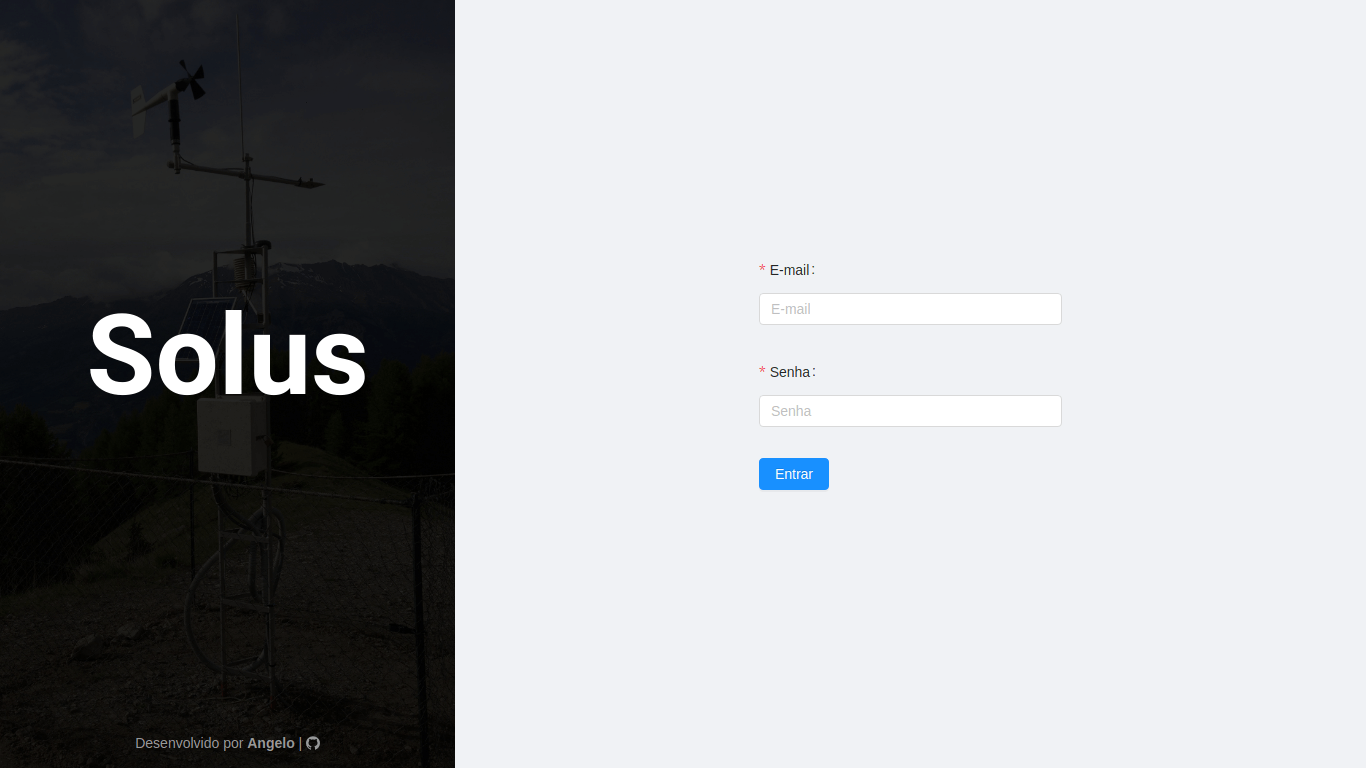
\includegraphics[scale=0.3]{telas/login.png}
    \hfill
\legend{Fonte: Produção do autor.}
\end{figure}

Na tela de login apresentada na figura \ref{fig:screen_login}, pode-se conferir o formulário de acesso ao sistema, requisitando o e-mail e senha do usuário e o botão de acesso, ao ser confirmado o login no sistema o usuário é levado até a tela principal do sistema.

\begin{figure}[H]
    \centering
    \caption{Dashboard} \label{fig:screen_filtros}
    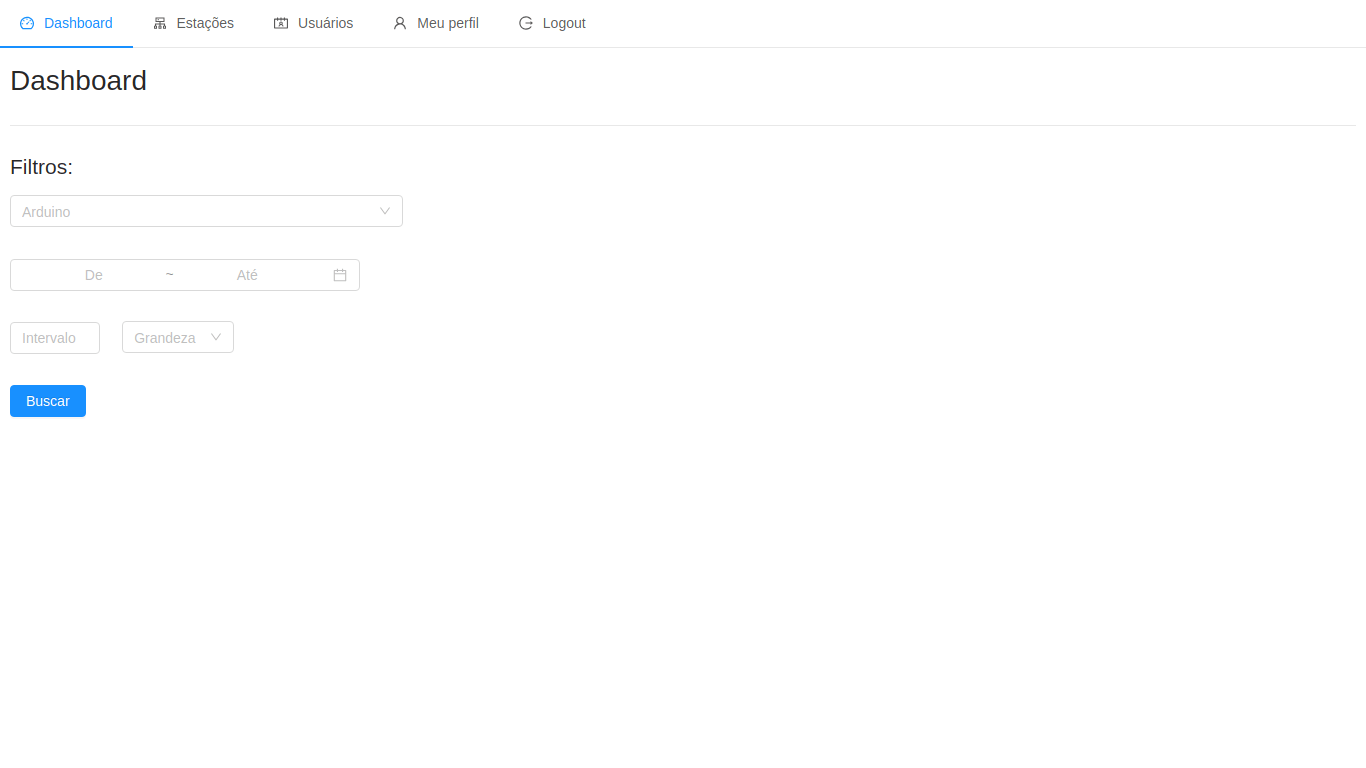
\includegraphics[scale=0.3]{telas/filtros.png}
    \hfill
\legend{Fonte: Produção do autor.}
\end{figure}

Conforme pode-se conferir na figura \ref{fig:screen_filtros} na tela inicial do sistema, pode-se conferir os filtros de dados, onde ao se escolher as informações de opção da estação meteorológica desejada, data inicial e data final de captura e qual o intervalo de tempo e confirmar a seleção de estatísticas, os resultados das figuras \ref{fig:screen_graphs1} a \ref{fig:screen_graphs3} são exibidos.

\begin{figure}[H]
    \centering
    \caption{Resultados de estatísticas \label{fig:screen_graphs1}}
    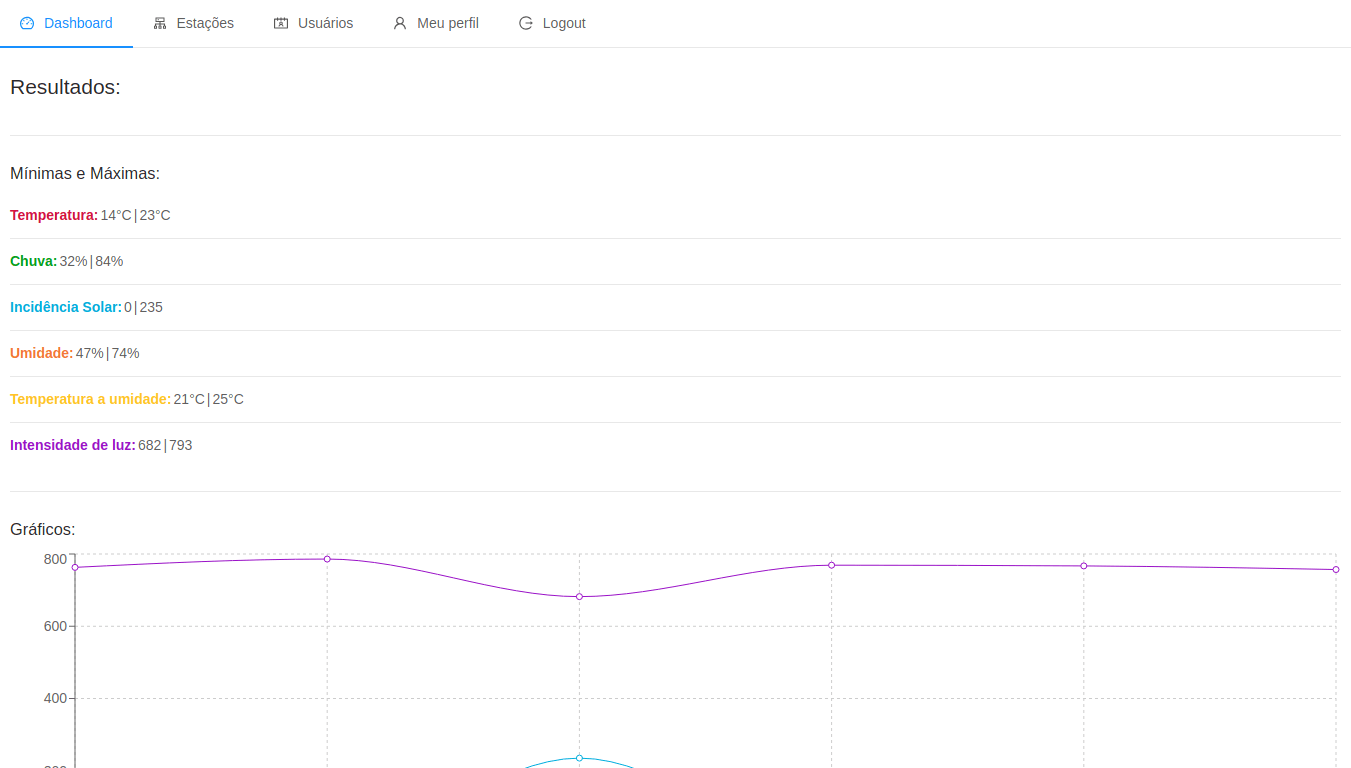
\includegraphics[scale=0.3]{telas/grafico1.png}
    \hfill
\legend{Fonte: Produção do autor.}
\end{figure}

\begin{figure}[H]
    \centering
    \caption{Gráficos das estatísticas \label{fig:screen_graphs2}}
    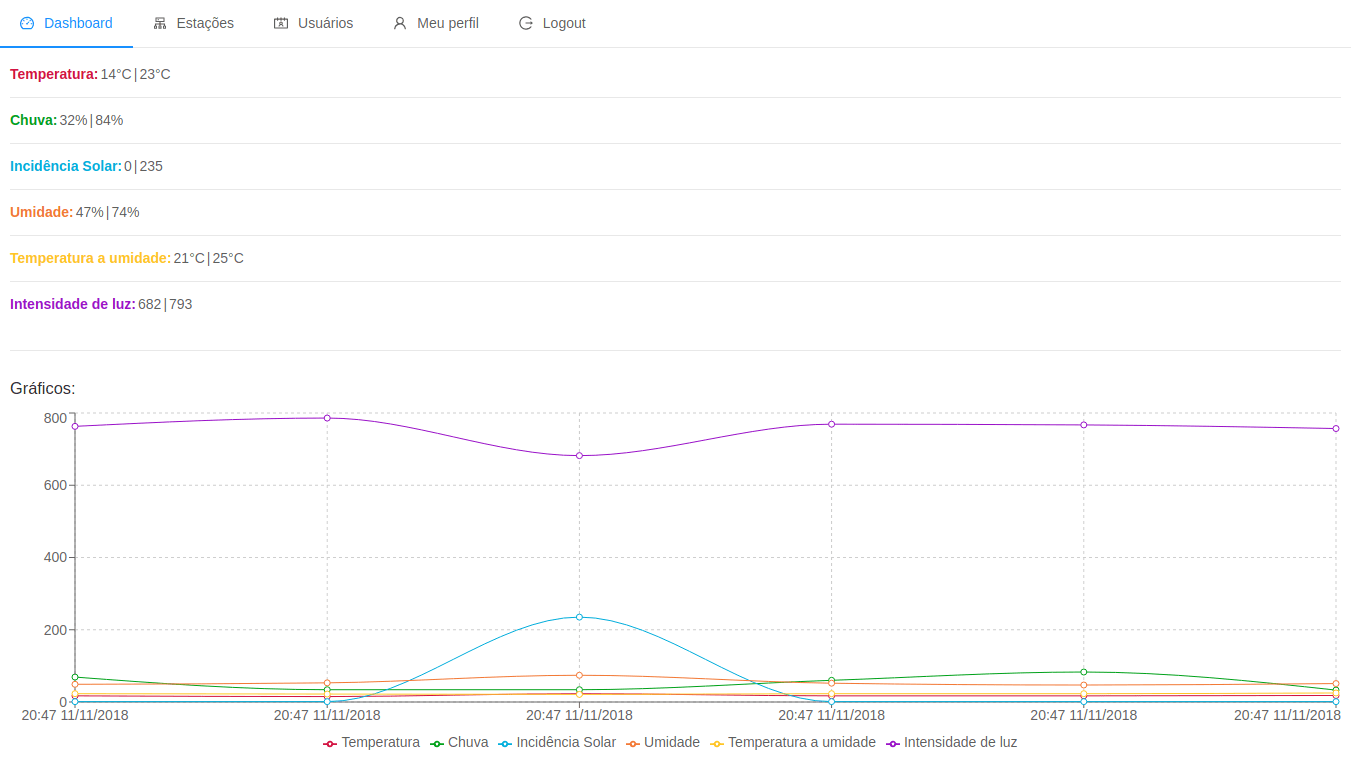
\includegraphics[scale=0.3]{telas/grafico2.png}
    \hfill
\legend{Fonte: Produção do autor.}
\end{figure}

\begin{figure}[H]
    \centering
    \caption{Números dos gráficos das estatísticas \label{fig:screen_graphs3}}
    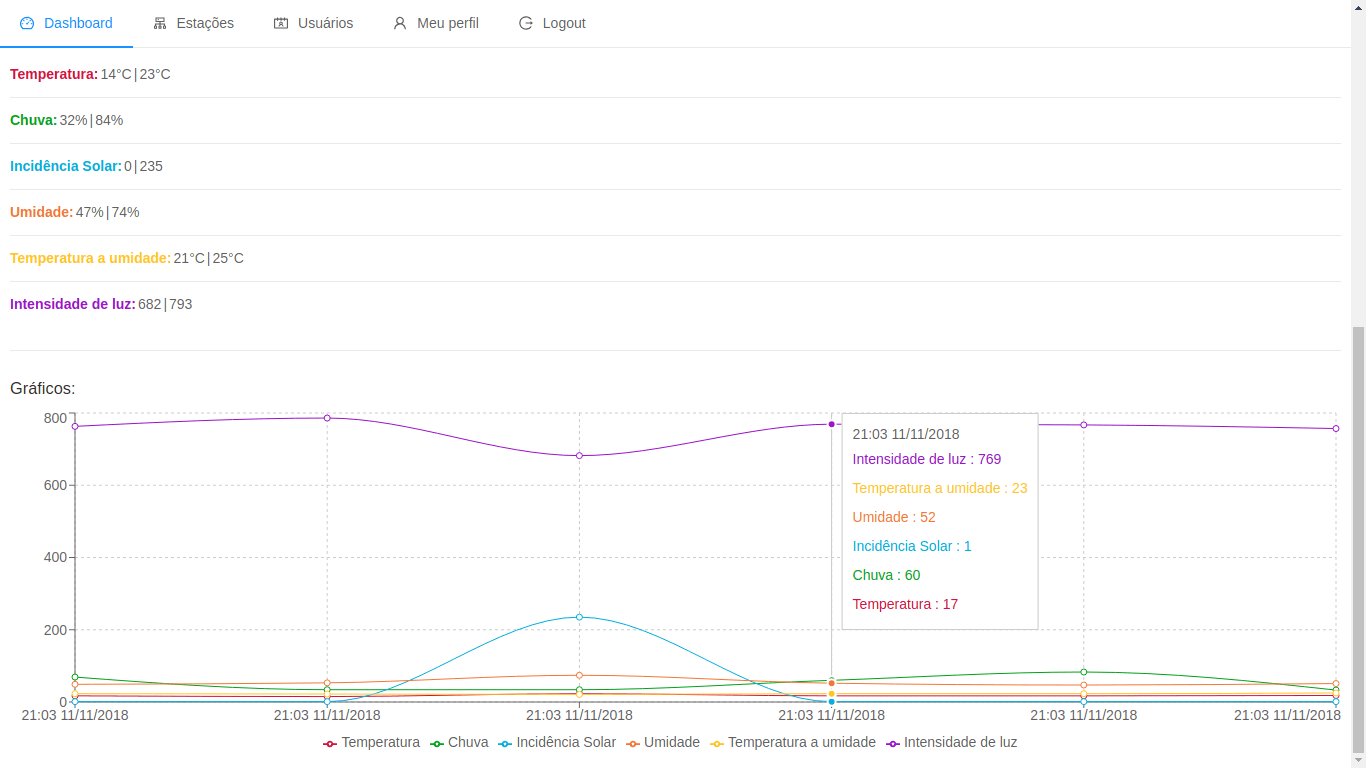
\includegraphics[scale=0.3]{telas/grafico3.png}
    \hfill
\legend{Fonte: Produção do autor.}
\end{figure}

São exibidas ao usuário as medidas de mínimas e máximas dos dados e os gráficos das médias que foram calculadas, conforme figuras \ref{fig:screen_graphs1} a \ref{fig:screen_graphs3}.

\begin{figure}[H]
    \centering
    \caption{Listagem de estações meteorológicas \label{fig:screen_estacoes}}
    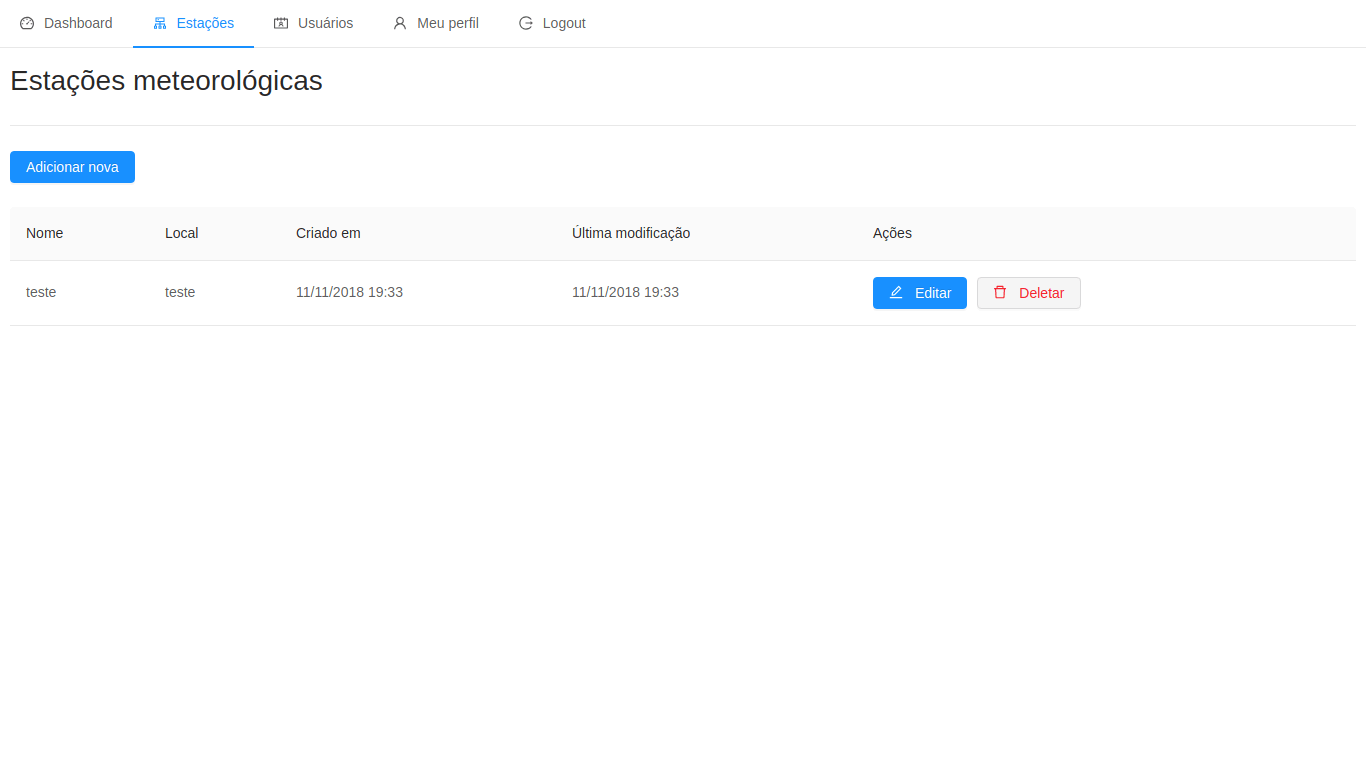
\includegraphics[scale=0.3]{telas/estacoes.png}
    \hfill
\legend{Fonte: Produção do autor.}
\end{figure}

Na listagem de estações meteorológicas (figura \ref{fig:screen_estacoes}), é exibida ao usuário uma tabela com as informações das estações meteorológicas cadastradas, há no topo da tabela a opção de adicionar uma nova estação meteorológica e para cada uma das linhas da tabela são exibidas as ações de editar ou excluir o registro de uma estação meteorológica, os modais de cadastro e edição podem ser conferidos na figura \ref{fig:estacoes_add}, porém, no caso da edição, o modal já abre com as informações preenchidas.

\begin{figure}[H]
    \centering
    \caption{Modal de adição e edição dos dados de uma estação \label{fig:estacoes_add}}
    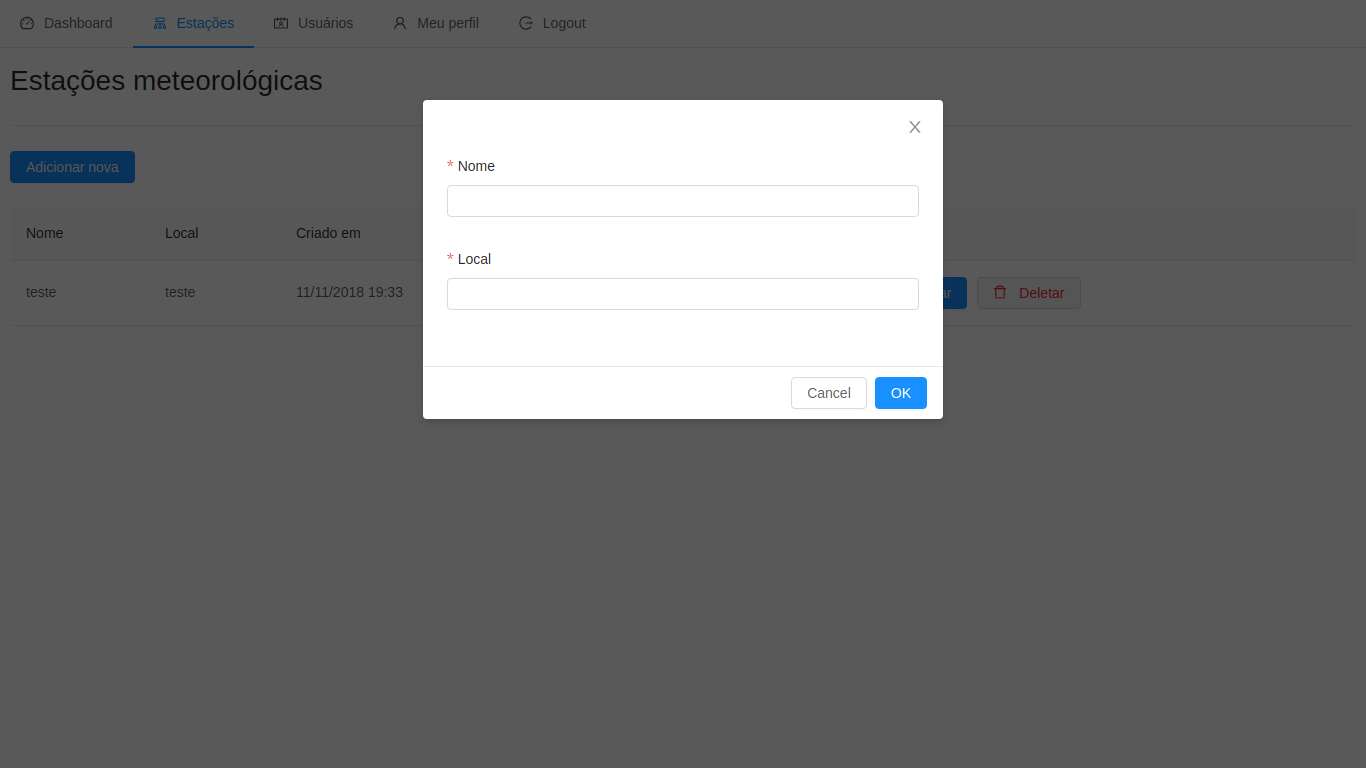
\includegraphics[scale=0.3]{telas/estacoes_add.png}
    \hfill
\legend{Fonte: Produção do autor.}
\end{figure}

\begin{figure}[H]
    \centering
    \caption{Listagem de usuários \label{fig:usuarios}}
    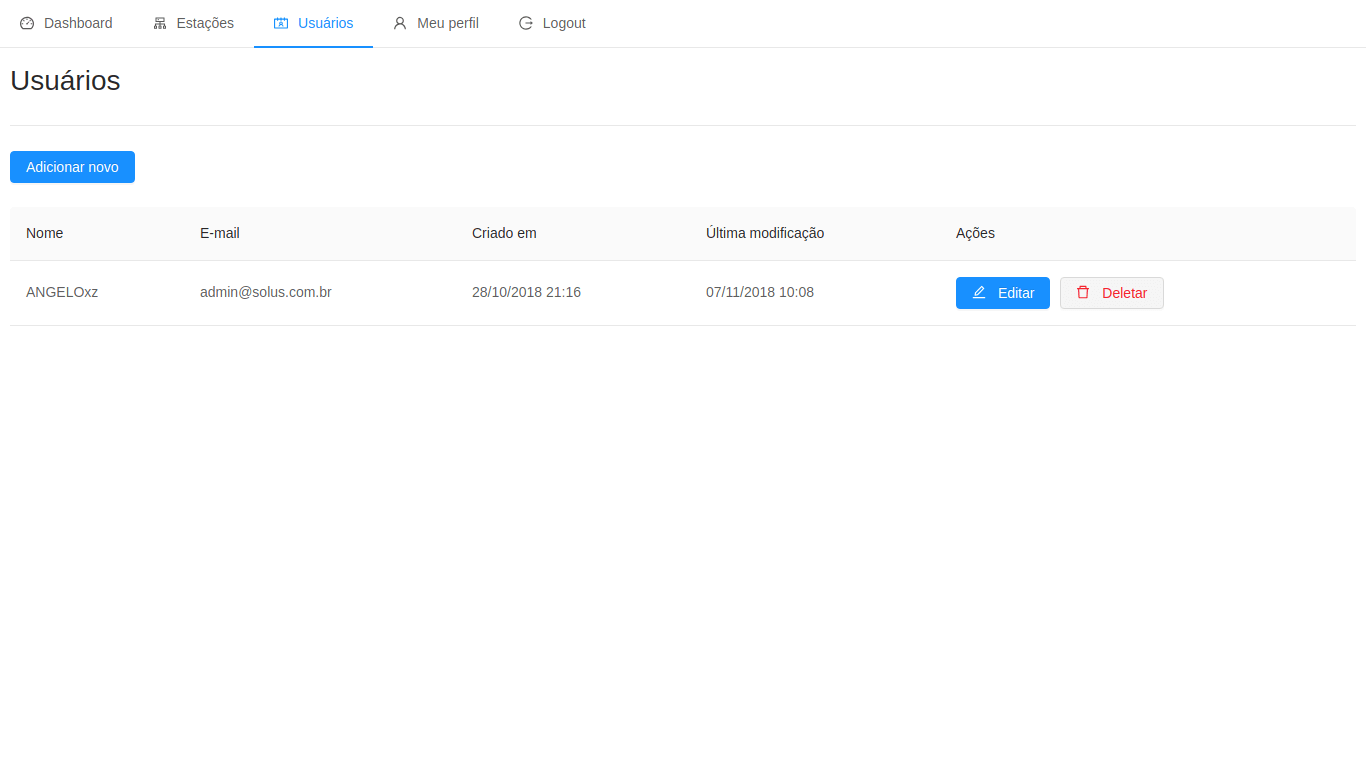
\includegraphics[scale=0.3]{telas/usuarios.png}
    \hfill
\legend{Fonte: Produção do autor.}
\end{figure}

A tela de listagem de usuários apresentada na figura \ref{fig:usuarios}, segue o mesmo comportamento da tela de listagem de estações meteorológicas, porém, para o modal de cadastro de usuário (Figura \ref{fig:usuarios_add}), é adicionado o campo opcional para edição de senha e e-mail.

\begin{figure}[H]
    \centering
    \caption{Modal de adição ou edição de usuário \label{fig:usuarios_add}}
    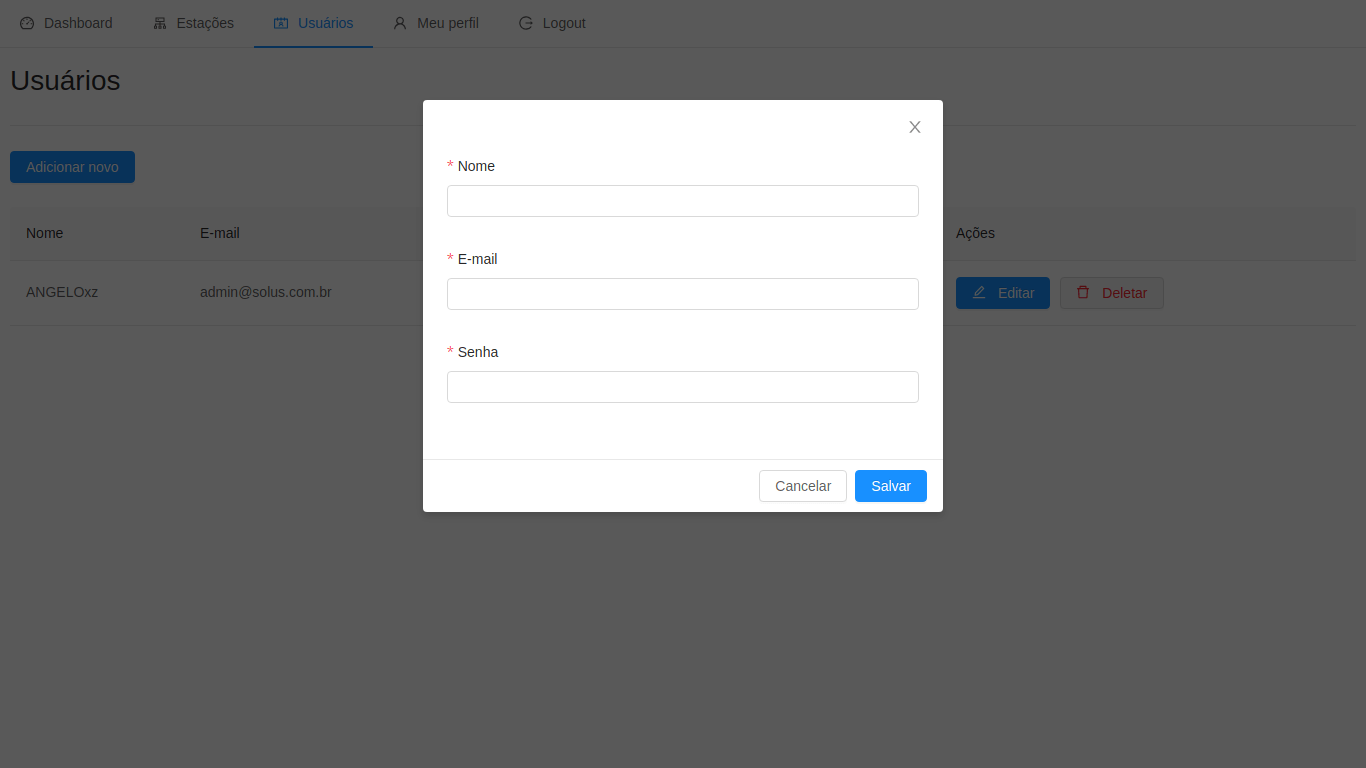
\includegraphics[scale=0.3]{telas/usuarios_add.png}
    \hfill
\legend{Fonte: Produção do autor.}
\end{figure}

\begin{figure}[H]
    \centering
    \caption{Visualização de meu perfil \label{fig:perfil}}
    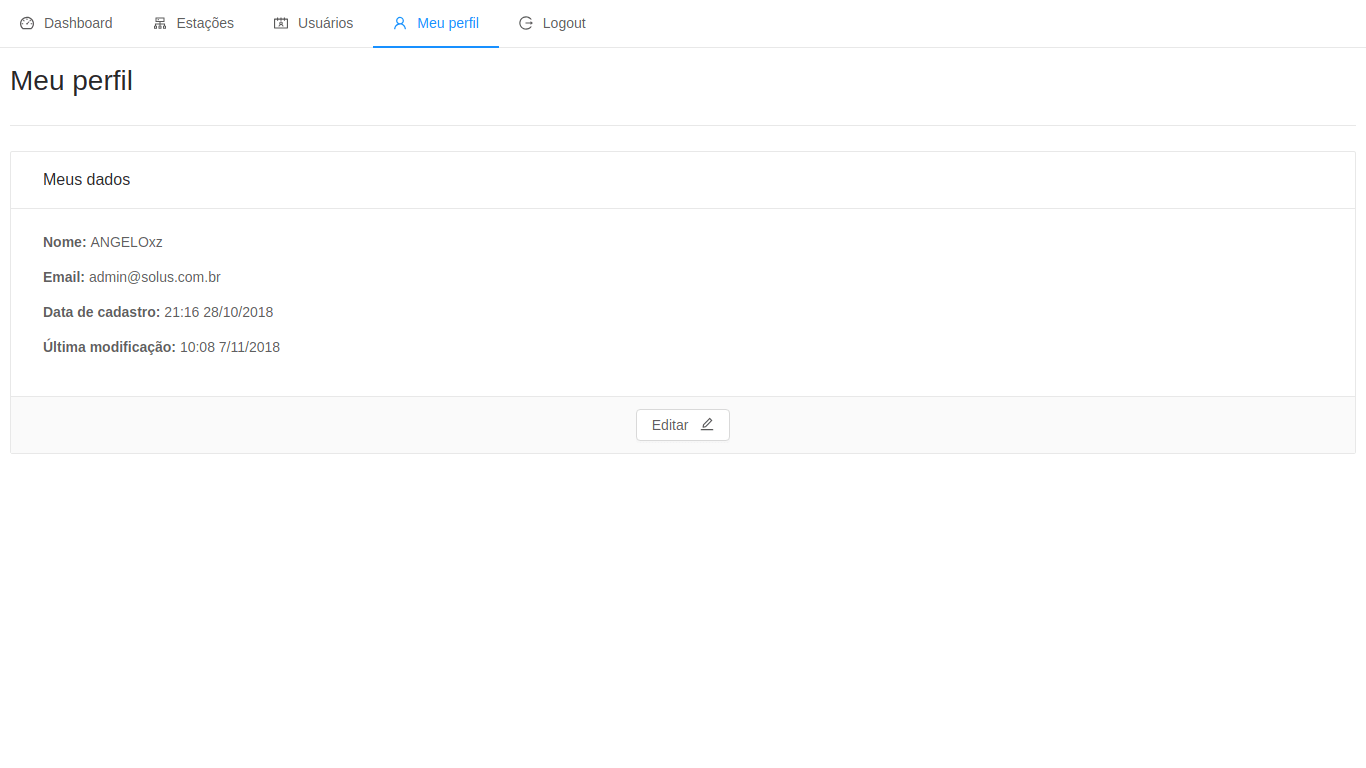
\includegraphics[scale=0.3]{telas/perfil.png}
    \hfill
\legend{Fonte: Produção do autor.}
\end{figure}

Na tela \textbf{Meu perfil}, conforme figura \ref{fig:perfil} são exibidos os dados do usuário que está utilizando o sistema no momento, caso o usuário abre a função de edição, é exibido o formulário conforme figura \ref{fig:perfil_edit}, que ao ser confirmado, é fechado novamente, exibindo somente suas informações já atualizadas.

\begin{figure}[H]
    \centering
    \caption{Edição de perfil \label{fig:perfil_edit}}
    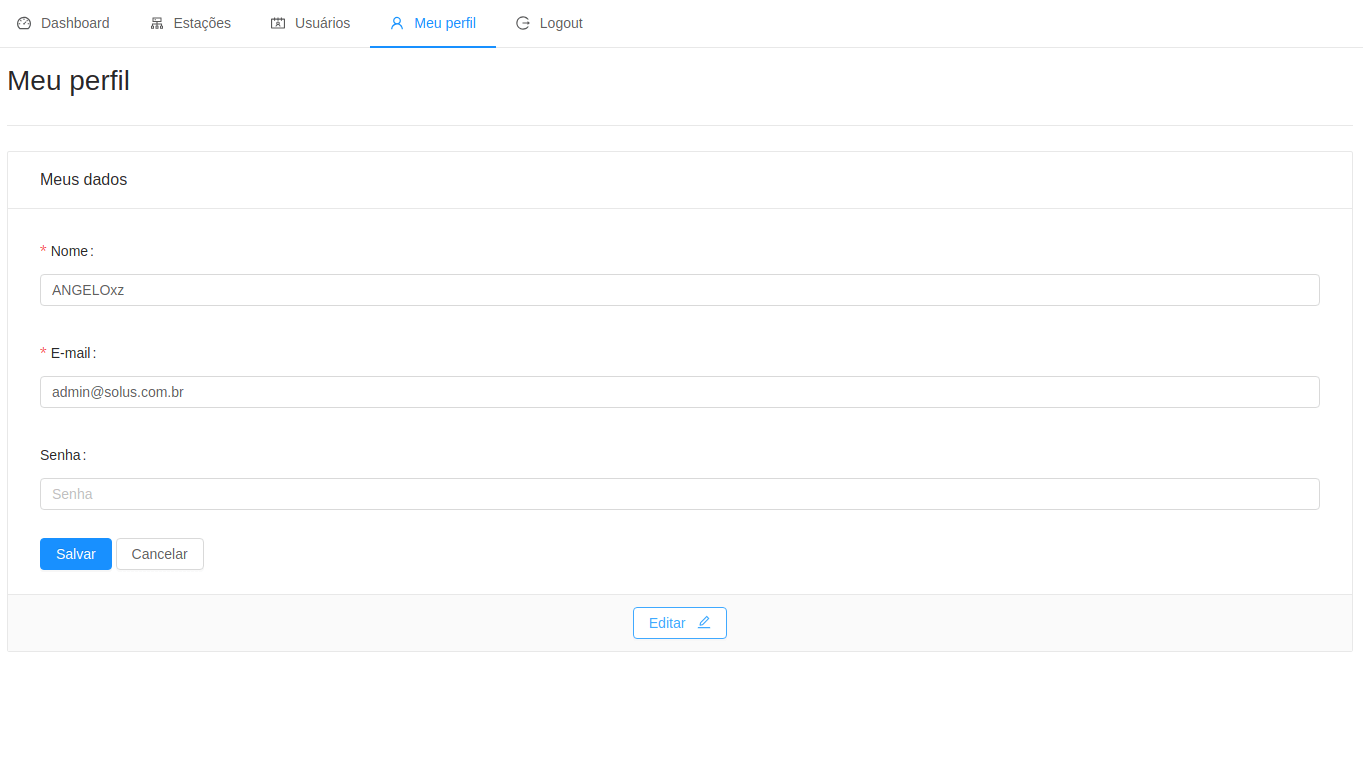
\includegraphics[scale=0.3]{telas/perfil_edit.png}
    \hfill
\legend{Fonte: Produção do autor.}
\end{figure}

% ----------------------------------------------------------
% Finaliza a parte no bookmark do PDF
% para que se inicie o bookmark na raiz
% e adiciona espaço de parte no Sumário
% ----------------------------------------------------------
\phantompart

\chapter{Conclusão}

Através da análise de dados utilizando métricas de mínima, máxima e média, foi possível visualizar mudanças climáticas que afetam a captação de energia solar, utilizando o sistema desenvolvido, o usuário pode tomar decisões acerca do posicionamento dos painéis solares, visando assim, mudanças que favorecem maior captação de energia solar através dos painéis fotovoltaicos.

O sistema desenvolvido é capaz de fornecer uma ferramenta ao especialista para análise e acompanhamento de informações importantes no acompanhamento de painéis solares, atingido assim seus objetivos.

Para projeto futuros, dadas as facilidades de mudança no software e na forma como os dados foram modelados, acrescentaria mais valor ao software, serem adicionadas novas medidas meteorológicas, enriquecendo mais a forma como o usuário é informado.

Medições importantes como a velocidade do vento e a quantidade em milímetros de chuva não foram adicionados, e trariam grandes avanços ao projeto. Funcionalidades geográficas como identificação das estações meteorológicas através de posicionamento em mapa seriam interessantes ferramentas para a análise meteorológica proposta.
